\hypertarget{biology-the-science-of-life}{%
\chapter{Biology: The Science of Life}\label{biology-the-science-of-life}}

\href{https://en.wikipedia.org/wiki/Biology}{Biology} is the natural
science that studies life and living organisms, including their physical
structure, chemical processes, molecular interactions, physiological
mechanisms, development and evolution. Despite the complexity of the
science, certain unifying concepts consolidate it into a single,
coherent field. Biology recognizes the cell as the basic unit of life,
genes as the basic unit of heredity, and evolution as the engine that
propels the creation and extinction of species. Living
\href{https://en.wikipedia.org/wiki/Organism}{organisms} (from Greek
ὀργανισμός, organismos, from ὄργανον, organon, i.e.~``instrument,
implement, tool, organ of sense or apprehension'') are open systems that
survive by transforming energy and decreasing their local entropy to
maintain a stable and vital condition defined as homeostasis.

\begin{figure}

{\centering 
\includegraphics[width=0.7\linewidth]{./figures/life/IMG_1024} 

}

\caption{A Common Eastern Bumble Bee (\emph{Bombus impatiens}) picking up nectar and pollen from a spear cistle (\emph{Cirsium vulgare}) on Winter Island in Salem, Massachusetts.}\label{fig:bumblebee}
\end{figure}

Sub-disciplines of biology are defined by the research methods employed and the kind of system studied: theoretical biology uses mathematical methods to formulate quantitative models while experimental biology performs empirical experiments to test the validity of proposed theories and understand the mechanisms underlying life and how it appeared and evolved from non-living matter about 4 billion years ago through a gradual increase in the complexity of the system.

Biology derives from the Ancient Greek words of βίος; romanized bíos meaning ``life'' and -λογία; romanized logía (-logy) meaning ``branch of study'' or ``to speak''. Those combined make the Greek word βιολογία; romanized biología meaning biology. Despite this, the term βιολογία as a whole didn't exist in Ancient Greek. The first to borrow it was the English and French (biologie). Since the advent of the scientific era, reanalyzable as a compound using the combining forms bio + logy.

The Latin-language form of the term first appeared in 1736 when Swedish scientist \href{https://en.wikipedia.org/wiki/Carl_Linnaeus}{Carl Linnaeus} (Carl von Linné) used biologi in his Bibliotheca Botanica. It was used again in 1766 in a work entitled Philosophiae naturalis sive physicae: tomus III, continens geologian, biologian, phytologian generalis, by Michael Christoph Hanov, a disciple of Christian Wolff. The first German use, Biologie, was in a 1771 translation of Linnaeus' work. In 1797, Theodor Georg August Roose used the term in the preface of a book, Grundzüge der Lehre van der Lebenskraft. Karl Friedrich Burdach used the term in 1800 in a more restricted sense of the study of human beings from a morphological, physiological and psychological perspective (Propädeutik zum Studien der gesammten Heilkunst). The term came into its modern usage with the six-volume treatise Biologie, oder Philosophie der lebenden Natur (1802--22) by Gottfried Reinhold Treviranus, who announced:

\begin{quote}
The objects of our research will be the different forms and manifestations of life, the conditions and laws under which these phenomena occur, and the causes through which they have been effected. The science that concerns itself with these objects we will indicate by the name biology {[}Biologie{]} or the doctrine of life {[}Lebenslehre{]}.
\end{quote}

Although modern biology is a relatively recent development, sciences related to and included within it have been studied since ancient times. Natural philosophy was studied as early as the ancient civilizations of Mesopotamia, Egypt, the Indian subcontinent, and China. However, the origins of modern biology and its approach to the study of nature are most often traced back to ancient Greece. While the formal study of medicine dates back to Pharaonic Egypt, it was Aristotle (384--322 BC) who contributed most extensively to the development of biology. Especially important are his History of Animals and other works where he showed naturalist leanings, and later more empirical works that focused on biological causation and the diversity of life. Aristotle's successor at the Lyceum, Theophrastus, wrote a series of books on botany that survived as the most important contribution of antiquity to the plant sciences, even into the Middle Ages.

Scholars of the medieval Islamic world who wrote on biology included al-Jahiz (781--869), Al-Dīnawarī (828--896), who wrote on botany, and Rhazes (865--925) who wrote on anatomy and physiology. Medicine was especially well studied by Islamic scholars working in Greek philosopher traditions, while natural history drew heavily on Aristotelian thought, especially in upholding a fixed hierarchy of life.

Biology began to quickly develop and grow with \href{https://en.wikipedia.org/wiki/Antonie_van_Leeuwenhoek}{Anton van Leeuwenhoek's} dramatic improvement of the microscope. It was then that scholars discovered spermatozoa, bacteria, infusoria and the diversity of microscopic life. Investigations by Jan Swammerdam led to new interest in entomology and helped to develop the basic techniques of microscopic dissection and staining.

Advances in microscopy also had a profound impact on biological thinking. In the early 19th century, a number of biologists pointed to the central importance of the cell. Then, in 1838, Schleiden and Schwann began promoting the now universal ideas that (1) the basic unit of organisms is the cell and (2) that individual cells have all the characteristics of life, although they opposed the idea that (3) all cells come from the division of other cells. Thanks to the work of Robert Remak and Rudolf Virchow, however, by the 1860s most biologists accepted all three tenets of what came to be known as cell theory.

Meanwhile, taxonomy and classification became the focus of natural historians. Carl Linnaeus published a basic taxonomy for the natural world in 1735 (variations of which have been in use ever since), and in the 1750s introduced scientific names for all his species. \href{https://en.wikipedia.org/wiki/Georges-Louis_Leclerc,_Comte_de_Buffon}{Georges-Louis Leclerc}, Comte de Buffon, treated species as artificial categories and living forms as malleable---even suggesting the possibility of common descent. Although he was opposed to evolution, Buffon is a key figure in the history of evolutionary thought; his work influenced the evolutionary theories of both Lamarck and Darwin.

Serious evolutionary thinking originated with the works of \href{https://en.wikipedia.org/wiki/Jean-Baptiste_Lamarck}{Jean-Baptiste Lamarck}, who was the first to present a coherent theory of evolution. He posited that evolution was the result of environmental stress on properties of animals, meaning that the more frequently and rigorously an organ was used, the more complex and efficient it would become, thus adapting the animal to its environment. Lamarck believed that these acquired traits could then be passed on to the animal's offspring, who would further develop and perfect them. However, it was the British naturalist \href{https://en.wikipedia.org/wiki/Charles_Darwin}{Charles Darwin}, combining the biogeographical approach of Humboldt, the uniformitarian geology of Lyell, Malthus's writings on population growth, and his own morphological expertise and extensive natural observations, who forged a more successful evolutionary theory based on natural selection; similar reasoning and evidence led \href{https://en.wikipedia.org/wiki/Alfred_Russel_Wallace}{Alfred Russel Wallace} to independently reach the same conclusions. Although it was the subject of controversy (which continues to this day), Darwin's theory quickly spread through the scientific community and soon became a central axiom of the rapidly developing science of biology.

The discovery of the physical representation of heredity came along with evolutionary principles and population genetics. In the 1940s and early 1950s, experiments pointed to DNA as the component of chromosomes that held the trait-carrying units that had become known as genes. A focus on new kinds of model organisms such as viruses and bacteria, along with the discovery of the double-helical structure of DNA in 1953, marked the transition to the era of molecular genetics. From the 1950s to the present times, biology has been vastly extended in the molecular domain. The genetic code was cracked by Har Gobind Khorana, Robert W. Holley and Marshall Warren Nirenberg after DNA was understood to contain codons. Finally, the Human Genome Project was launched in 1990 with the goal of mapping the general human genome. This project was essentially completed in 2003, with further analysis still being published. The Human Genome Project was the first step in a globalized effort to incorporate accumulated knowledge of biology into a functional, molecular definition of the human body and the bodies of other organisms.

\hypertarget{characteristics-of-life}{%
\section{Characteristics of Life}\label{characteristics-of-life}}

In the past, there have been many attempts to define what is meant by ``life'' through obsolete concepts such as odic force, hylomorphism, spontaneous generation and vitalism, that have now been disproved by biological discoveries. Aristotle is considered to be the first person to classify organisms. Later, Carl Linnaeus introduced his system of binomial nomenclature for the classification of species. Eventually new groups and categories of life were discovered, such as cells and microorganisms, forcing dramatic revisions of the structure of relationships between living organisms. Though currently only known on Earth, life need not be restricted to it, and many scientists speculate in the existence of extraterrestrial life. Artificial life is a computer simulation or human-made reconstruction of any aspect of life, which is often used to examine systems related to natural life.

Death is the permanent termination of all biological functions which sustain an organism, and as such, is the end of its life. Extinction is the term describing the dying out of a group or taxon, usually a species. Fossils are the preserved remains or traces of organisms.

The definition of life has long been a challenge for scientists and philosophers, with many varied definitions put forward. This is partially because life is a process, not a substance. This is complicated by a lack of knowledge of the characteristics of living entities, if any, that may have developed outside of Earth. Philosophical definitions of life have also been put forward, with similar difficulties on how to distinguish living things from the non-living. Legal definitions of life have also been described and debated, though these generally focus on the decision to declare a human dead, and the legal ramifications of this decision.

Since there is no unequivocal definition of life, most current definitions in biology are descriptive. Life is considered a characteristic of something that preserves, furthers or reinforces its existence in the given environment. This characteristic exhibits all or most of the following traits:

\begin{itemize}
\tightlist
\item
  Homeostasis: regulation of the internal environment to maintain a constant state; for example, sweating to reduce temperature
\item
  Organization: being structurally composed of one or more cells -- the basic units of life
\item
  Metabolism: transformation of energy by converting chemicals and energy into cellular components (anabolism) and decomposing organic matter (catabolism). Living things require energy to maintain internal organization (homeostasis) and to produce the other phenomena associated with life.
\item
  Growth: maintenance of a higher rate of anabolism than catabolism. A growing organism increases in size in all of its parts, rather than simply accumulating matter.
\item
  Adaptation: the ability to change over time in response to the environment. This ability is fundamental to the process of evolution and is determined by the organism's heredity, diet, and external factors.
\item
  Response to stimuli: a response can take many forms, from the contraction of a unicellular organism to external chemicals, to complex reactions involving all the senses of multicellular organisms. A response is often expressed by motion; for example, the leaves of a plant turning toward the sun (phototropism), and chemotaxis.
\item
  Reproduction: the ability to produce new individual organisms, either asexually from a single parent organism or sexually from two parent organisms.
\end{itemize}

These complex processes, called physiological functions, have underlying physical and chemical bases, as well as signaling and control mechanisms that are essential to maintaining life.

More than 99\% of all species of life forms, amounting to over five billion species, that ever lived on Earth are estimated to be extinct.

Although the number of Earth's catalogued species of lifeforms is between 1.2 million and 2 million, the total number of species in the planet is uncertain. Estimates range from 8 million to 100 million, with a more narrow range between 10 and 14 million, but it may be as high as 1 trillion (with only one-thousandth of one percent of the species described) according to studies realized in May 2016. The total number of related DNA base pairs on Earth is estimated at 5.0 x 10\textsuperscript{37} and weighs 50 billion tonnes. In comparison, the total mass of the biosphere has been estimated to be as much as 4 TtC (trillion tons of carbon). In July 2016, scientists reported identifying a set of 355 genes from the Last Universal Common Ancestor (LUCA) of all organisms living on Earth.

\hypertarget{origin-of-life}{%
\section{Origin of Life}\label{origin-of-life}}

The Ancient Greeks believed that living things could spontaneously come into being from nonliving matter, and that the goddess Gaia could make life arise spontaneously from stones -- a process known as Generatio spontanea. \href{https://en.wikipedia.org/wiki/Aristotle}{Aristotle} disagreed, but he still believed that creatures could arise from dissimilar organisms or from soil. Variations of this concept of spontaneous generation still existed as late as the 17th century, but towards the end of the 17th century, a series of observations and arguments began that eventually discredited such ideas. This advance in scientific understanding was met with much opposition, with personal beliefs and individual prejudices often obscuring the facts.

\href{https://en.wikipedia.org/wiki/William_Harvey}{William Harvey} (1578--1657) was an early proponent of all life beginning from an egg, omne vivum ex ovo. \href{https://en.wikipedia.org/wiki/Francesco_Redi}{Francesco Redi}, an Italian physician, proved as early as 1668 that higher forms of life did not originate spontaneously by demonstrating that maggots come from eggs of flies. But proponents of spontaneous generation claimed that this did not apply to microbes and continued to hold that these could arise spontaneously. Attempts to disprove the spontaneous generation of life from non-life continued in the early 19th century with observations and experiments by Franz Schulze and \href{https://en.wikipedia.org/wiki/Theodor_Schwann}{Theodor Schwann}. In 1745, \href{https://en.wikipedia.org/wiki/John_Needham}{John Needham} added chicken broth to a flask and boiled it. He then let it cool and waited. Microbes grew, and he proposed it as an example of spontaneous generation. In 1768, \href{https://en.wikipedia.org/wiki/Lazzaro_Spallanzani}{Lazzaro Spallanzani} repeated Needham's experiment but removed all the air from the flask. No growth occurred. In 1854, Heinrich G. F. Schröder (1810--1885) and Theodor von Dusch, and in 1859, Schröder alone, repeated the Helmholtz filtration experiment and showed that living particles can be removed from air by filtering it through cotton-wool.

In 1864, \href{https://en.wikipedia.org/wiki/Louis_Pasteur}{Louis Pasteur} finally announced the results of his scientific experiments. In a series of experiments similar to those performed earlier by Needham and Spallanzani, Pasteur demonstrated that life does not arise in areas that have not been contaminated by existing life. Pasteur's empirical results were summarized in the phrase Omne vivum ex vivo, Latin for ``all life {[}is{]} from life''.

All known life forms share fundamental molecular mechanisms, reflecting their common descent; based on these observations, hypotheses on the origin of life attempt to find a mechanism explaining the formation of a universal common ancestor, from simple organic molecules via pre-cellular life to protocells and metabolism. Models have been divided into ``genes-first'' and ``metabolism-first'' categories, but a recent trend is the emergence of hybrid models that combine both categories.

Life on Earth is based on carbon and water. Carbon provides stable frameworks for complex chemicals and can be easily extracted from the environment, especially from carbon dioxide. There is no other chemical element whose properties are similar enough to carbon's to be called an analogue; silicon, the element directly below carbon on the periodic table, does not form very many complex stable molecules, and because most of its compounds are water-insoluble and because silicon dioxide is a hard and abrasive solid in contrast to carbon dioxide at temperatures associated with living things, it would be more difficult for organisms to extract. The elements boron and phosphorus have more complex chemistries, but suffer from other limitations relative to carbon. Water is an excellent solvent and has two other useful properties: the fact that ice floats enables aquatic organisms to survive beneath it in winter; and its molecules have electrically negative and positive ends, which enables it to form a wider range of compounds than other solvents can. Other good solvents, such as ammonia, are liquid only at such low temperatures that chemical reactions may be too slow to sustain life, and lack water's other advantages. Organisms based on alternative biochemistry may, however, be possible on other planets.

\href{https://en.wikipedia.org/wiki/Abiogenesis}{Abiogenesis}, or informally the origin of life, is the natural process of life arising from non-living matter, such as simple organic compounds. The prevailing scientific hypothesis is that the transition from non-living to living entities was not a single event, but a gradual process of increasing complexity. Although the occurrence of abiogenesis is uncontroversial among scientists, its possible mechanisms are poorly understood. There are several principles and hypotheses for how abiogenesis could have occurred. Life on Earth first appeared as early as 4.28 billion years ago, soon after ocean formation 4.41 billion years ago, and not long after the formation of the Earth 4.54 billion years ago. The earliest known life forms are microfossils of bacteria.

There is no current scientific consensus as to how life originated. However, many accepted scientific models build on the Miller--Urey experiment and the work of Sidney Fox, which show that conditions on the primitive Earth favored chemical reactions that synthesize amino acids and other organic compounds from inorganic precursors, and phospholipids spontaneously form lipid bilayers, the basic structure of a cell membrane.

The classic 1952 Miller--Urey experiment (Figure \ref{fig:millerurey}) demonstrated that most amino acids, the chemical constituents of the proteins used in all living organisms, can be synthesized from inorganic compounds under conditions intended to replicate those of the early Earth. The experiment used water (H\textsubscript{2}O), methane (CH\textsubscript{4}), ammonia (NH\textsubscript{3}), and hydrogen (H\textsubscript{2}). The chemicals were all sealed inside a sterile 5-liter glass flask connected to a 500 ml flask half-full of water. The water in the smaller flask was heated to induce evaporation, and the water vapour was allowed to enter the larger flask. Continuous electrical sparks were fired between the electrodes to simulate lightning in the water vapour and gaseous mixture, and then the simulated atmosphere was cooled again so that the water condensed and trickled into a U-shaped trap at the bottom of the apparatus.

After a day, the solution collected at the trap had turned pink in colour, and after a week of continuous operation the solution was deep red and turbid. The boiling flask was then removed, and mercuric chloride was added to prevent microbial contamination. The reaction was stopped by adding barium hydroxide and sulfuric acid, and evaporated to remove impurities. Using paper chromatography, Miller identified five amino acids present in the solution: glycine, α-alanine and β-alanine were positively identified, while aspartic acid and α-aminobutyric acid (AABA) were less certain, due to the spots being faint.Complex organic molecules occur in the Solar System and in interstellar space, and these molecules may have provided starting material for the development of life on Earth.



\begin{figure}

{\centering 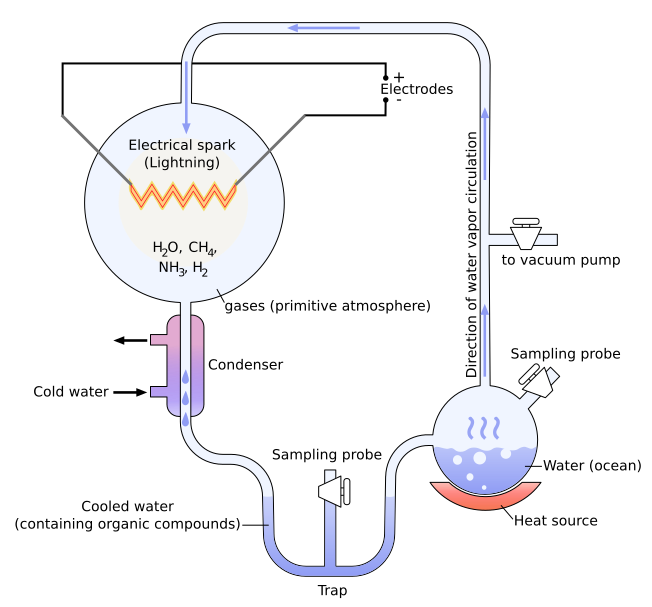
\includegraphics[width=0.7\linewidth]{./figures/life/Miller-Urey_experiment-en} 

}

\caption{\href{https://commons.wikimedia.org/wiki/File:MUexperiment.png}{The Miller--Urey experiment} was a chemical experiment that simulated the conditions thought at the time (1952) to be present on the early Earth and tested the chemical origin of life under those conditions. The experiment at the time supported Alexander Oparin's and J. B. S. Haldane's hypothesis that putative conditions on the primitive Earth favoured chemical reactions that synthesized more complex organic compounds from simpler inorganic precursors. Considered to be the classic experiment investigating abiogenesis, it was conducted in 1952 by Stanley Miller, with assistance from Harold Urey, at the University of Chicago and later the University of California, San Diego and published the following year.}\label{fig:millerurey}
\end{figure}

Living organisms synthesize proteins, which are polymers of amino acids using instructions encoded by deoxyribonucleic acid (DNA). Protein synthesis entails intermediary ribonucleic acid (RNA) polymers. One possibility for how life began is that genes originated first, followed by proteins; the alternative being that proteins came first and then genes.

However, because genes and proteins are both required to produce the other, the problem of considering which came first is like that of the chicken or the egg. Most scientists have adopted the hypothesis that because of this, it is unlikely that genes and proteins arose independently.

Therefore, a possibility, first suggested by Francis Crick, is that the first life was based on RNA, which has the DNA-like properties of information storage and the catalytic properties of some proteins. This is called the RNA world hypothesis, and it is supported by the observation that many of the most critical components of cells (those that evolve the slowest) are composed mostly or entirely of RNA. Also, many critical cofactors (ATP, Acetyl-CoA, NADH, etc.) are either nucleotides or substances clearly related to them. The catalytic properties of RNA had not yet been demonstrated when the hypothesis was first proposed, but they were confirmed by Thomas Cech in 1986.

One issue with the RNA world hypothesis is that synthesis of RNA from simple inorganic precursors is more difficult than for other organic molecules. One reason for this is that RNA precursors are very stable and react with each other very slowly under ambient conditions, and it has also been proposed that living organisms consisted of other molecules before RNA. However, the successful synthesis of certain RNA molecules under the conditions that existed prior to life on Earth has been achieved by adding alternative precursors in a specified order with the precursor phosphate present throughout the reaction. This study makes the RNA world hypothesis more plausible.

Geological findings in 2013 showed that reactive phosphorus species (like phosphite) were in abundance in the ocean before 3.5 Ga, and that Schreibersite easily reacts with aqueous glycerol to generate phosphite and glycerol 3-phosphate. It is hypothesized that Schreibersite-containing meteorites from the Late Heavy Bombardment could have provided early reduced phosphorus, which could react with prebiotic organic molecules to form phosphorylated biomolecules, like RNA.

In 2009, experiments demonstrated Darwinian evolution of a two-component system of RNA enzymes (ribozymes) in vitro. The work was performed in the laboratory of Gerald Joyce, who stated ``This is the first example, outside of biology, of evolutionary adaptation in a molecular genetic system.''

Prebiotic compounds may have originated extraterrestrially. NASA findings in 2011, based on studies with meteorites found on Earth, suggest DNA and RNA components (adenine, guanine and related organic molecules) may be formed in outer space.

In March 2015, NASA scientists reported that, for the first time, complex DNA and RNA organic compounds of life, including uracil, cytosine and thymine, have been formed in the laboratory under outer space conditions, using starting chemicals, such as pyrimidine, found in meteorites. Pyrimidine, like polycyclic aromatic hydrocarbons (PAHs), the most carbon-rich chemical found in the universe, may have been formed in red giants or in interstellar dust and gas clouds, according to the scientists.

According to the panspermia hypothesis, microscopic life---distributed by meteoroids, asteroids and other small Solar System bodies---may exist throughout the universe.

Since its primordial beginnings, life on Earth has changed its environment on a geologic time scale, but it has also adapted to survive in most ecosystems and conditions. Some microorganisms, called extremophiles, thrive in physically or geochemically extreme environments that are detrimental to most other life on Earth. The cell is considered the structural and functional unit of life. There are two kinds of cells, prokaryotic and eukaryotic, both of which consist of cytoplasm enclosed within a membrane and contain many biomolecules such as proteins and nucleic acids. Cells reproduce through a process of cell division, in which the parent cell divides into two or more daughter cells.



\begin{figure}

{\centering 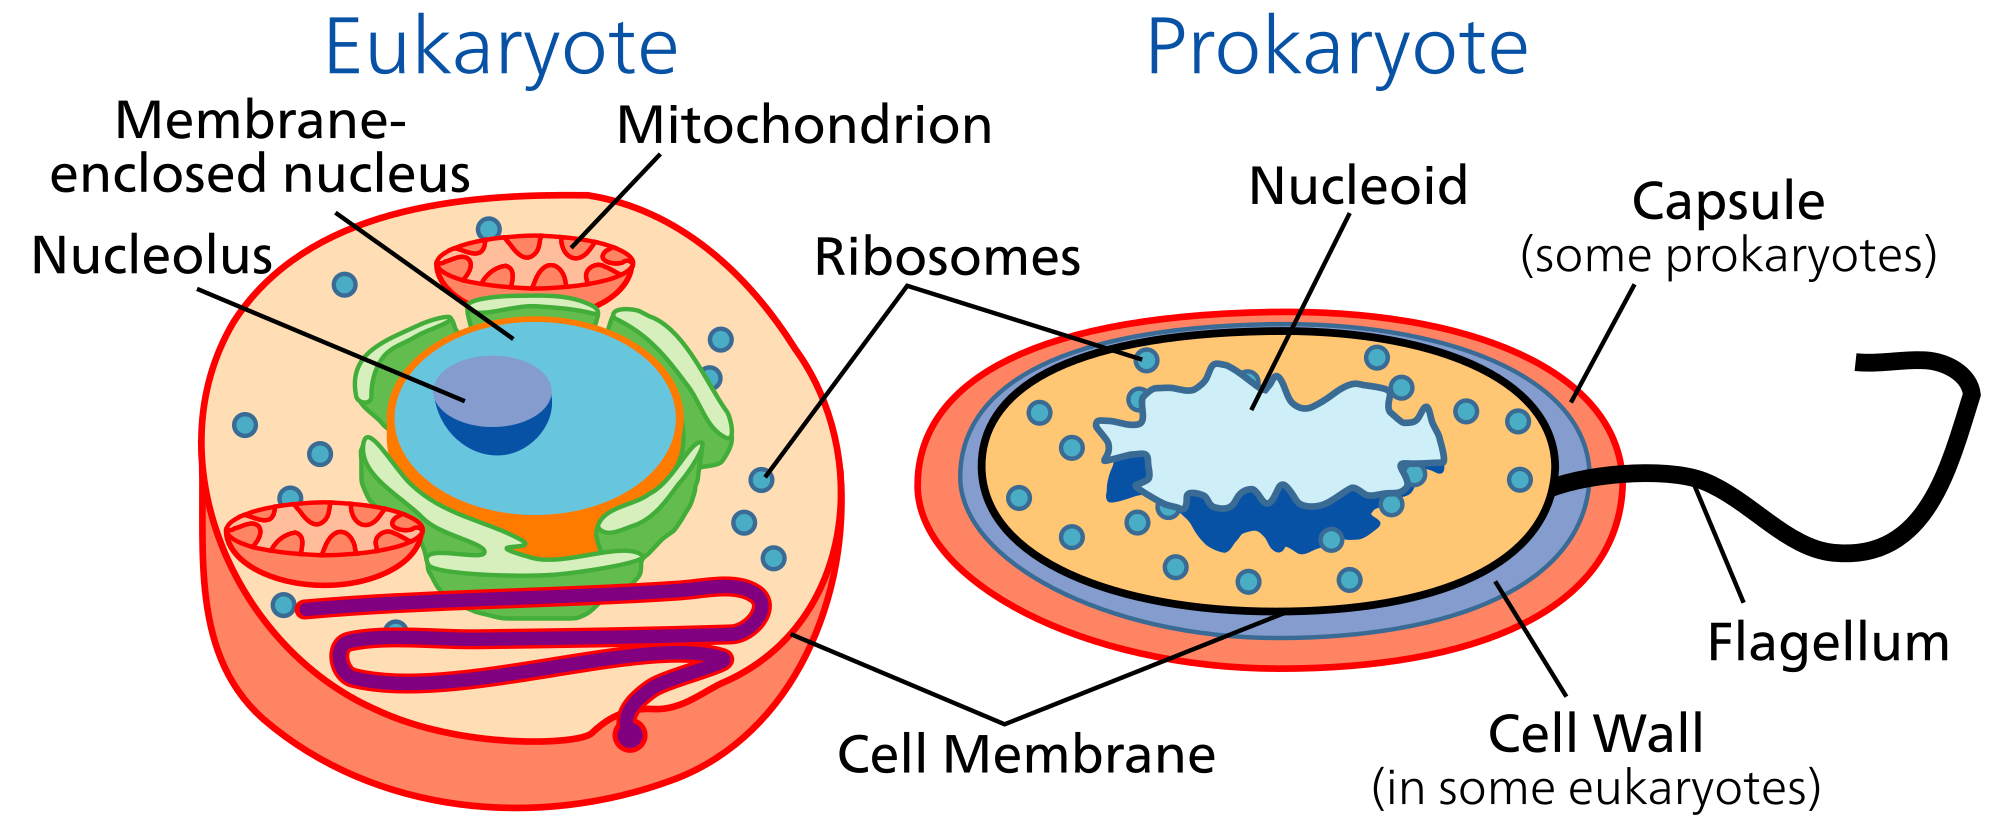
\includegraphics[width=0.7\linewidth]{./figures/life/Celltypes} 

}

\caption{\href{https://commons.wikimedia.org/wiki/File:Celltypes.svg}{Cartoons of a eukaryotic and prokaryotic cell.}}\label{fig:celltypecartoon}
\end{figure}

\hypertarget{foundations-of-modern-biology}{%
\section{Foundations of Modern Biology}\label{foundations-of-modern-biology}}

\hypertarget{cell-theory}{%
\subsection{Cell theory}\label{cell-theory}}

\href{https://en.wikipedia.org/wiki/Cell_theory}{Cell theory} states that the cell is the fundamental unit of life, that all living things are composed of one or more cells, and that all cells arise from pre-existing cells through cell division. In multicellular organisms, every cell in the organism's body derives ultimately from a single cell in a fertilized egg. The cell is also considered to be the basic unit in many pathological processes. In addition, the phenomenon of energy flow occurs in cells in processes that are part of the function known as metabolism. Finally, cells contain hereditary information (DNA), which is passed from cell to cell during cell division. Research into the origin of life, abiogenesis, amounts to an attempt to discover the origin of the first cells.

Cells are the basic unit of structure in every living thing, and all cells arise from pre-existing cells by division. Cell theory was formulated by Henri Dutrochet, Theodor Schwann, Rudolf Virchow and others during the early nineteenth century, and subsequently became widely accepted. The activity of an organism depends on the total activity of its cells, with energy flow occurring within and between them. Cells contain hereditary information that is carried forward as a genetic code during cell division.

There are two primary types of cells. \href{https://en.wikipedia.org/wiki/Prokaryote}{Prokaryotes} lack a nucleus and other membrane-bound organelles, although they have circular DNA and ribosomes. \href{https://en.wikipedia.org/wiki/Bacteria}{Bacteria} and \href{https://en.wikipedia.org/wiki/Archaea}{Archaea} are two domains of prokaryotes. The other primary type of cells are the \href{https://en.wikipedia.org/wiki/Eukaryote}{eukaryotes}, which have distinct nuclei bound by a nuclear membrane and membrane-bound organelles, including mitochondria, chloroplasts, lysosomes, rough and smooth endoplasmic reticulum, and vacuoles. In addition, they possess organized chromosomes that store genetic material. All species of large complex organisms are eukaryotes, including animals, plants and fungi, though most species of eukaryote are protist microorganisms. The conventional model is that eukaryotes evolved from prokaryotes, with the main organelles of the eukaryotes forming through endosymbiosis between bacteria and the progenitor eukaryotic cell.



\begin{figure}

{\centering 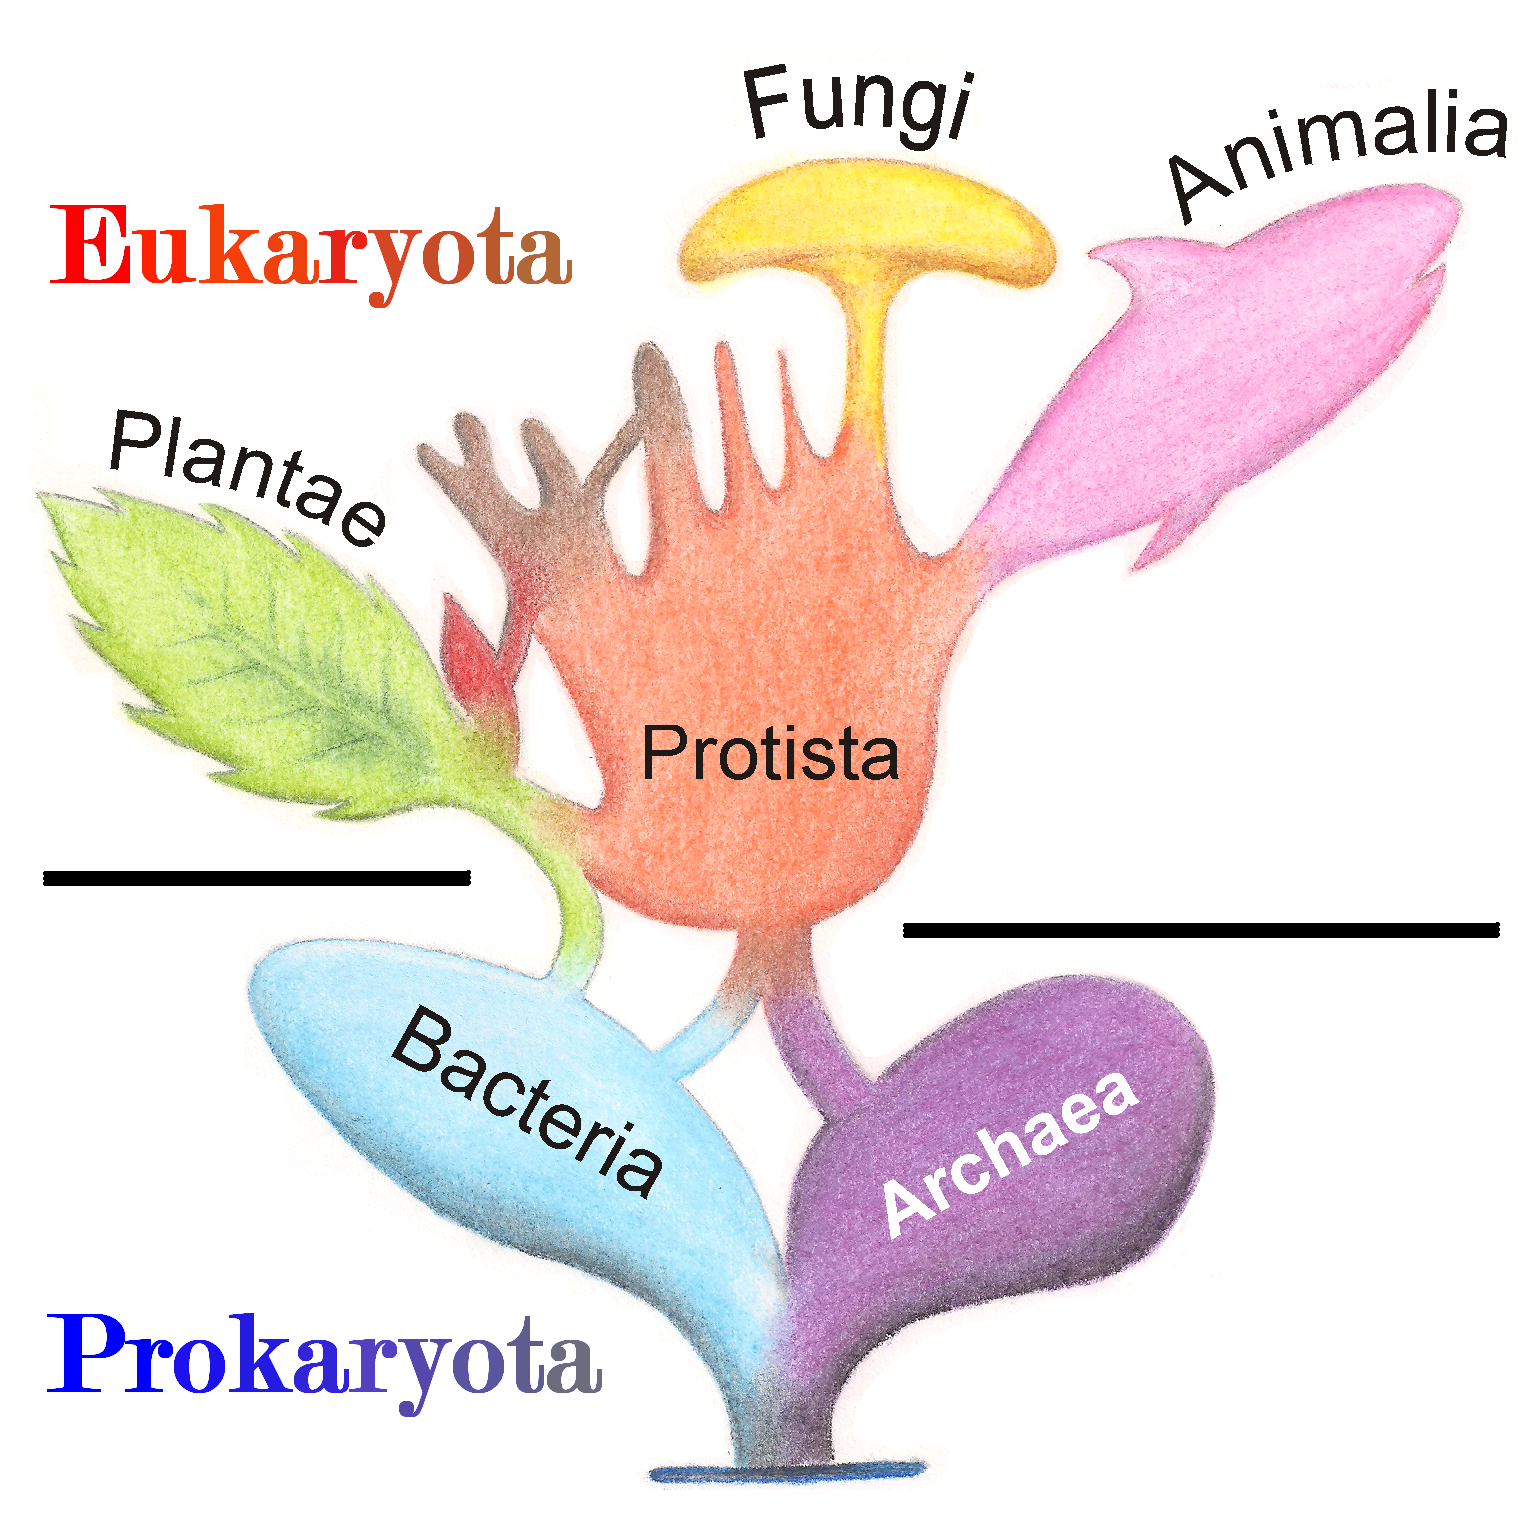
\includegraphics[width=0.7\linewidth]{./figures/life/Tree_of_Living_Organisms_2} 

}

\caption{\href{https://commons.wikimedia.org/wiki/File:Tree_of_Living_Organisms_2.png}{Tree diagram} illustrating the evolutionary relationship of living organisms{]}}\label{fig:livorgtree}
\end{figure}

A \href{https://en.wikipedia.org/wiki/Virus}{virus} is a submicroscopic infectious agent that replicates only inside the living cells of an organism. Scientific opinions differ on whether viruses are a form of life, or organic structures that interact with living organisms. They have been described as ``organisms at the edge of life'', since they resemble organisms in that they possess genes, evolve by natural selection, and reproduce by creating multiple copies of themselves through self-assembly. Although they have genes, they do not have a cellular structure, which is seen as the basic unit of life. Viruses do not have their own metabolism, and require a host cell to make new products. They therefore cannot naturally reproduce outside a host cell---although bacterial species such as rickettsia and chlamydia are considered living organisms despite the same limitation. Accepted forms of life use cell division to reproduce, whereas viruses spontaneously assemble within cells. They differ from autonomous growth of crystals as they inherit genetic mutations while being subject to natural selection. Virus self-assembly within host cells has implications for the study of the origin of life, as it lends further credence to the hypothesis that life could have started as self-assembling organic molecules.

The molecular mechanisms of cell biology are based on proteins which are synthesized by the ribosomes through an enzyme-catalyzed process called protein biosynthesis. A sequence of amino acids is assembled and joined together based upon gene expression of the cell's nucleic acid. In eukaryotic cells, these proteins may then be transported and processed through the Golgi apparatus in preparation for dispatch to their destination.

Cells reproduce through a process of cell division in which the parent cell divides into two or more daughter cells. For prokaryotes, cell division occurs through a process of fission in which the DNA is replicated, then the two copies are attached to parts of the cell membrane. In eukaryotes, a more complex process of mitosis is followed. However, the end result is the same; the resulting cell copies are identical to each other and to the original cell (except for mutations), and both are capable of further division following an interphase period.

Multicellular organisms may have first evolved through the formation of colonies of identical cells. These cells can form group organisms through cell adhesion. The individual members of a colony are capable of surviving on their own, whereas the members of a true multi-cellular organism have developed specializations, making them dependent on the remainder of the organism for survival. Such organisms are formed clonally or from a single germ cell that is capable of forming the various specialized cells that form the adult organism. This specialization allows multicellular organisms to exploit resources more efficiently than single cells. In January 2016, scientists reported that, about 800 million years ago, a minor genetic change in a single molecule, called GK-PID, may have allowed organisms to go from a single cell organism to one of many cells.

Cells have evolved methods to perceive and respond to their microenvironment, thereby enhancing their adaptability. Cell signaling coordinates cellular activities, and hence governs the basic functions of multicellular organisms. Signaling between cells can occur through direct cell contact using juxtacrine signalling, or indirectly through the exchange of agents as in the endocrine system. In more complex organisms, coordination of activities can occur through a dedicated nervous system.

\hypertarget{the-theory-of-evolution}{%
\subsection{The Theory of Evolution}\label{the-theory-of-evolution}}

A central organizing concept in biology is that life changes and develops through \href{https://en.wikipedia.org/wiki/Evolution}{evolution}, and that all life-forms known have a common origin. The theory of evolution postulates that all organisms on the Earth, both living and extinct, have descended from a common ancestor or an ancestral gene pool. This universal common ancestor of all organisms is believed to have appeared about 3.5 billion years ago. Biologists regard the ubiquity of the genetic code as definitive evidence in favor of the theory of universal common descent for all bacteria, archaea, and eukaryotes.

The term ``evolution'' was introduced into the scientific lexicon by \href{https://en.wikipedia.org/wiki/Jean-Baptiste_Lamarck}{Jean-Baptiste de Lamarck} in 1809, and fifty years later \href{https://en.wikipedia.org/wiki/Charles_Darwin}{Charles Darwin} posited a scientific model of natural selection as evolution's driving force. \href{https://en.wikipedia.org/wiki/Alfred_Russel_Wallace}{Alfred Russel Wallace} independently reached the same conclusions and is recognized as the co-discoverer of this concept. Evolution is now used to explain the great variations of life found on Earth.

Darwin theorized that species flourish or die when subjected to the processes of natural selection or selective breeding. Genetic drift was embraced as an additional mechanism of evolutionary development in the modern synthesis of the theory.

The evolutionary history of the species---which describes the characteristics of the various species from which it descended---together with its genealogical relationship to every other species is known as its phylogeny. Widely varied approaches to biology generate information about phylogeny. These include the comparisons of DNA sequences, a product of molecular biology (more particularly genomics), and comparisons of fossils or other records of ancient organisms, a product of paleontology. Biologists organize and analyze evolutionary relationships through various methods, including phylogenetics, phenetics, and cladistics

Evolution is relevant to the understanding of the natural history of life forms and to the understanding of the organization of current life forms. But, those organizations can only be understood in light of how they came to be by way of the process of evolution. Consequently, evolution is central to all fields of biology.

The evolutionary history of life on Earth traces the processes by which living and fossil organisms evolved, from the earliest emergence of life to the present. Earth formed about 4.5 billion years (Ga) ago and evidence suggests life emerged prior to 3.7 Ga. (Although there is some evidence of life as early as 4.1 to 4.28 Ga, it remains controversial due to the possible non-biological formation of the purported fossils.) The similarities among all known present-day species indicate that they have diverged through the process of evolution from a common ancestor. Approximately 1 trillion species currently live on Earth of which only 1.75--1.8 million have been named and 1.6 million documented in a central database. These currently living species represent less than one percent of all species that have ever lived on earth.

The earliest evidence of life comes from biogenic carbon signatures and stromatolite fossils discovered in 3.7 billion-year-old metasedimentary rocks from western Greenland. In 2015, possible ``remains of biotic life'' were found in 4.1 billion-year-old rocks in Western Australia. In March 2017, putative evidence of possibly the oldest forms of life on Earth was reported in the form of fossilized microorganisms discovered in hydrothermal vent precipitates in the Nuvvuagittuq Belt of Quebec, Canada, that may have lived as early as 4.28 billion years ago, not long after the oceans formed 4.4 billion years ago, and not long after the formation of the Earth 4.54 billion years ago.



\begin{figure}

{\centering 
\includegraphics[width=0.7\linewidth]{./figures/life/Stromatolites_in_Sharkbay} 

}

\caption{\href{https://commons.wikimedia.org/wiki/File:Stromatolites_in_Sharkbay.jpg}{Modern stromatolites in Shark Bay, Western Australia}}\label{fig:stromatolites}
\end{figure}

Microbial mats of coexisting bacteria and archaea were the dominant form of life in the early Archean Epoch and many of the major steps in early evolution are thought to have taken place in this environment. The evolution of photosynthesis, around 3.5 Ga, eventually led to a buildup of its waste product, oxygen, in the atmosphere, leading to the great oxygenation event, beginning around 2.4 Ga. The earliest evidence of eukaryotes (complex cells with organelles) dates from 1.85 Ga, and while they may have been present earlier, their diversification accelerated when they started using oxygen in their metabolism. Later, around 1.7 Ga, multicellular organisms began to appear, with differentiated cells performing specialised functions. Sexual reproduction, which involves the fusion of male and female reproductive cells (gametes) to create a zygote in a process called fertilization is, in contrast to asexual reproduction, the primary method of reproduction for the vast majority of macroscopic organisms, including almost all eukaryotes (which includes animals and plants). However the origin and evolution of sexual reproduction remain a puzzle for biologists though it did evolve from a common ancestor that was a single celled eukaryotic species. Bilateria, animals having a left and a right side that are mirror images of each other, appeared by 555 Ma (million years ago).

The earliest plants on land date back to around 850 million years ago (Ma), from carbon isotopes in Precambrian rocks, while algae-like multicellular land plants are dated back even to about 1 billion years ago, although evidence suggests that microorganisms formed the earliest terrestrial ecosystems, at least 2.7 billion years ago (Ga). Microorganisms are thought to have paved the way for the inception of land plants in the Ordovician. Land plants were so successful that they are thought to have contributed to the Late Devonian extinction event. (The long causal chain implied seems to involve the success of early tree archaeopteris (1) drew down CO\textsubscript{2} levels, leading to global cooling and lowered sea levels, (2) roots of archeopteris fostered soil development which increased rock weathering, and the subsequent nutrient run-off may have triggered algal blooms resulting in anoxic events which caused marine-life die-offs. Marine species were the primary victims of the Late Devonian extinction.)

Ediacara biota appear during the Ediacaran period, while vertebrates, along with most other modern phyla originated about 525 Ma during the Cambrian explosion. During the Permian period, synapsids, including the ancestors of mammals, dominated the land, but most of this group became extinct in the Permian--Triassic extinction event 252 Ma. During the recovery from this catastrophe, archosaurs became the most abundant land vertebrates; one archosaur group, the dinosaurs, dominated the Jurassic and Cretaceous periods. After the Cretaceous--Paleogene extinction event 65 Ma killed off the non-avian dinosaurs, mammals increased rapidly in size and diversity. Such mass extinctions may have accelerated evolution by providing opportunities for new groups of organisms to diversify.

\hypertarget{genetics}{%
\subsection{Genetics}\label{genetics}}

\href{https://en.wikipedia.org/wiki/Gene}{Genes} are the primary units of inheritance in all organisms. A gene is a unit of heredity and corresponds to a region of DNA that influences the form or function of an organism in specific ways. All organisms, from bacteria to animals, share the same basic machinery that copies and translates DNA into proteins. Cells transcribe a DNA gene into an RNA version of the gene, and a ribosome then translates the RNA into a sequence of amino acids known as a protein. The translation code from RNA codon to amino acid is the same for most organisms. For example, a sequence of DNA that codes for insulin in humans also codes for insulin when inserted into other organisms, such as plants.

\href{https://en.wikipedia.org/wiki/DNA}{DNA} is found as linear chromosomes in eukaryotes, and circular chromosomes in prokaryotes. A chromosome is an organized structure consisting of DNA and histones. The set of chromosomes in a cell and any other hereditary information found in the mitochondria, chloroplasts, or other locations is collectively known as a cell's genome. In eukaryotes, genomic DNA is localized in the cell nucleus, or with small amounts in mitochondria and chloroplasts. In prokaryotes, the DNA is held within an irregularly shaped body in the cytoplasm called the nucleoid. The genetic information in a genome is held within genes, and the complete assemblage of this information in an organism is called its genotype.

\hypertarget{homeostasis}{%
\subsection{Homeostasis}\label{homeostasis}}

\href{https://en.wikipedia.org/wiki/Homeostasis}{Homeostasis} is the ability of an open system to regulate its internal environment to maintain stable conditions by means of multiple dynamic equilibrium adjustments that are controlled by interrelated regulation mechanisms. All living organisms, whether unicellular or multicellular, exhibit homeostasis.

To maintain dynamic equilibrium and effectively carry out certain functions, a system must detect and respond to perturbations. After the detection of a perturbation, a biological system normally responds through negative feedback that stabilize conditions by reducing or increasing the activity of an organ or system. One example is the release of glucagon when sugar levels are too low.

\hypertarget{energy}{%
\subsection{Energy}\label{energy}}

The survival of a living organism depends on the continuous input of \href{https://en.wikipedia.org/wiki/Energy}{energy}. Chemical reactions that are responsible for its structure and function are tuned to extract energy from substances that act as its food and transform them to help form new cells and sustain them. In this process, molecules of chemical substances that constitute food play two roles; first, they contain energy that can be transformed and reused in that organism's biological, chemical reactions; second, food can be transformed into new molecular structures (biomolecules) that are of use to that organism.

The organisms responsible for the introduction of energy into an ecosystem are known as producers or autotrophs. Nearly all such organisms originally draw their energy from the sun. Plants and other phototrophs use solar energy via a process known as photosynthesis to convert raw materials into organic molecules, such as ATP, whose bonds can be broken to release energy. A few ecosystems, however, depend entirely on energy extracted by chemotrophs from methane, sulfides, or other non-luminal energy sources.

Some of the energy thus captured produces biomass and energy that is available for growth and development of other life forms. The majority of the rest of this biomass and energy are lost as waste molecules and heat. The most important processes for converting the energy trapped in chemical substances into energy useful to sustain life are metabolism and cellular respiration.

\hypertarget{areas-and-levels-of-study-and-research-in-biology}{%
\section{Areas And Levels of Study And Research in Biology}\label{areas-and-levels-of-study-and-research-in-biology}}

\href{https://en.wikipedia.org/wiki/Molecular_biology}{Molecular biology} is the study of biology at the molecular level. This field overlaps with other areas of biology, particularly those of genetics and biochemistry. Molecular biology is a study of the interactions of the various systems within a cell, including the interrelationships of DNA, RNA, and protein synthesis and how those interactions are regulated.

The next larger scale, \href{https://en.wikipedia.org/wiki/Cell_biology}{cell biology}, studies the structural and physiological properties of cells, including their internal behavior, interactions with other cells, and with their environment. This is done on both the microscopic and molecular levels, for unicellular organisms such as bacteria, as well as the specialized cells of multicellular organisms such as humans. Understanding the structure and function of cells is fundamental to all of the biological sciences. The similarities and differences between cell types are particularly relevant to molecular biology.

\href{https://en.wikipedia.org/wiki/Anatomy}{Anatomy} is a treatment of the macroscopic forms of such structures organs and organ systems.

\href{https://en.wikipedia.org/wiki/Genetics}{Genetics} is the science of genes, heredity, and the variation of organisms. Genes encode the information needed by cells for the synthesis of proteins, which in turn play a central role in influencing the final phenotype of the organism. Genetics provides research tools used in the investigation of the function of a particular gene, or the analysis of genetic interactions. Within organisms, genetic information is physically represented as chromosomes, within which it is represented by a particular sequence of amino acids in particular DNA molecules.

\href{https://en.wikipedia.org/wiki/Developmental_biology}{Developmental biology} studies the process by which organisms grow and develop. Developmental biology, originated from embryology, studies the genetic control of cell growth, cellular differentiation, and ``cellular morphogenesis,'' which is the process that progressively gives rise to tissues, organs, and anatomy. Model organisms for developmental biology include the round worm Caenorhabditis elegans, the fruit fly Drosophila melanogaster, the zebrafish Danio rerio, the mouse Mus musculus, and the weed Arabidopsis thaliana. (A model organism is a species that is extensively studied to understand particular biological phenomena, with the expectation that discoveries made in that organism provide insight into the workings of other organisms.)

\href{https://en.wikipedia.org/wiki/Physiology}{Physiology} is the study of the mechanical, physical, and biochemical processes of living organisms function as a whole. The theme of ``structure to function'' is central to biology. Physiological studies have traditionally been divided into plant physiology and animal physiology, but some principles of physiology are universal, no matter what particular organism is being studied. For example, what is learned about the physiology of yeast cells can also apply to human cells. The field of animal physiology extends the tools and methods of human physiology to non-human species. Plant physiology borrows techniques from both research fields.

\href{https://en.wikipedia.org/wiki/Evolutionary_biology}{Evolutionary biology} is concerned with the origin and descent of species, and their change over time. It employs scientists from many taxonomically oriented disciplines, for example, those with special training in particular organisms such as mammalogy, ornithology, botany, or herpetology, but are of use in answering more general questions about evolution.

Evolutionary biology is partly based on \href{https://en.wikipedia.org/wiki/Paleontology}{paleontology}, which uses the fossil record to answer questions about the mode and tempo of evolution, and partly on the developments in areas such as population genetics. In the 1980s, developmental biology re-entered evolutionary biology after its initial exclusion from the modern synthesis through the study of evolutionary developmental biology. Phylogenetics, systematics, and taxonomy are related fields often considered part of evolutionary biology.

Multiple speciation events create a tree structured system of relationships between species. The role of \href{https://en.wikipedia.org/wiki/Systematics}{systematics} is to study these relationships and thus the differences and similarities between species and groups of species. However, systematics was an active field of research long before evolutionary thinking was common.

Traditionally, living things have been divided into five kingdoms: Monera; Protista; Fungi; Plantae; Animalia. However, many scientists now consider this five-kingdom system outdated. Modern alternative classification systems generally begin with the three-domain system: Archaea (originally Archaebacteria); Bacteria (originally Eubacteria) and Eukaryota (including protists, fungi, plants, and animals). These domains reflect whether the cells have nuclei or not, as well as differences in the chemical composition of key biomolecules such as ribosomes.



\begin{figure}

{\centering 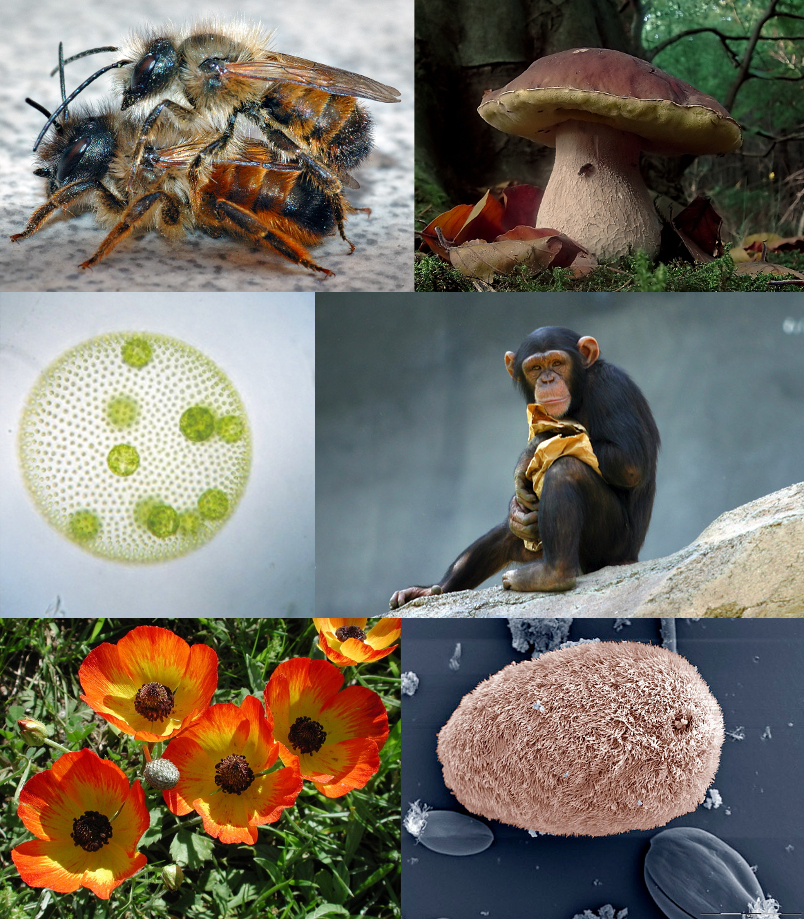
\includegraphics[width=0.7\linewidth]{./figures/life/Eukaryota_diversity_2} 

}

\caption{\href{https://commons.wikimedia.org/wiki/File:Eukaryota_diversity_2.jpg}{Eukaryotes and some examples of their diversity} -- clockwise from top left: Red mason bee, Boletus edulis, chimpanzee, Isotricha intestinalis, Ranunculus asiaticus, and Volvox carteri.}\label{fig:eukaryotediversity}
\end{figure}

Further, each kingdom is broken down recursively until each species is separately classified. The order is: Domain; Kingdom; Phylum; Class; Order; Family; Genus; Species.



\begin{figure}

{\centering 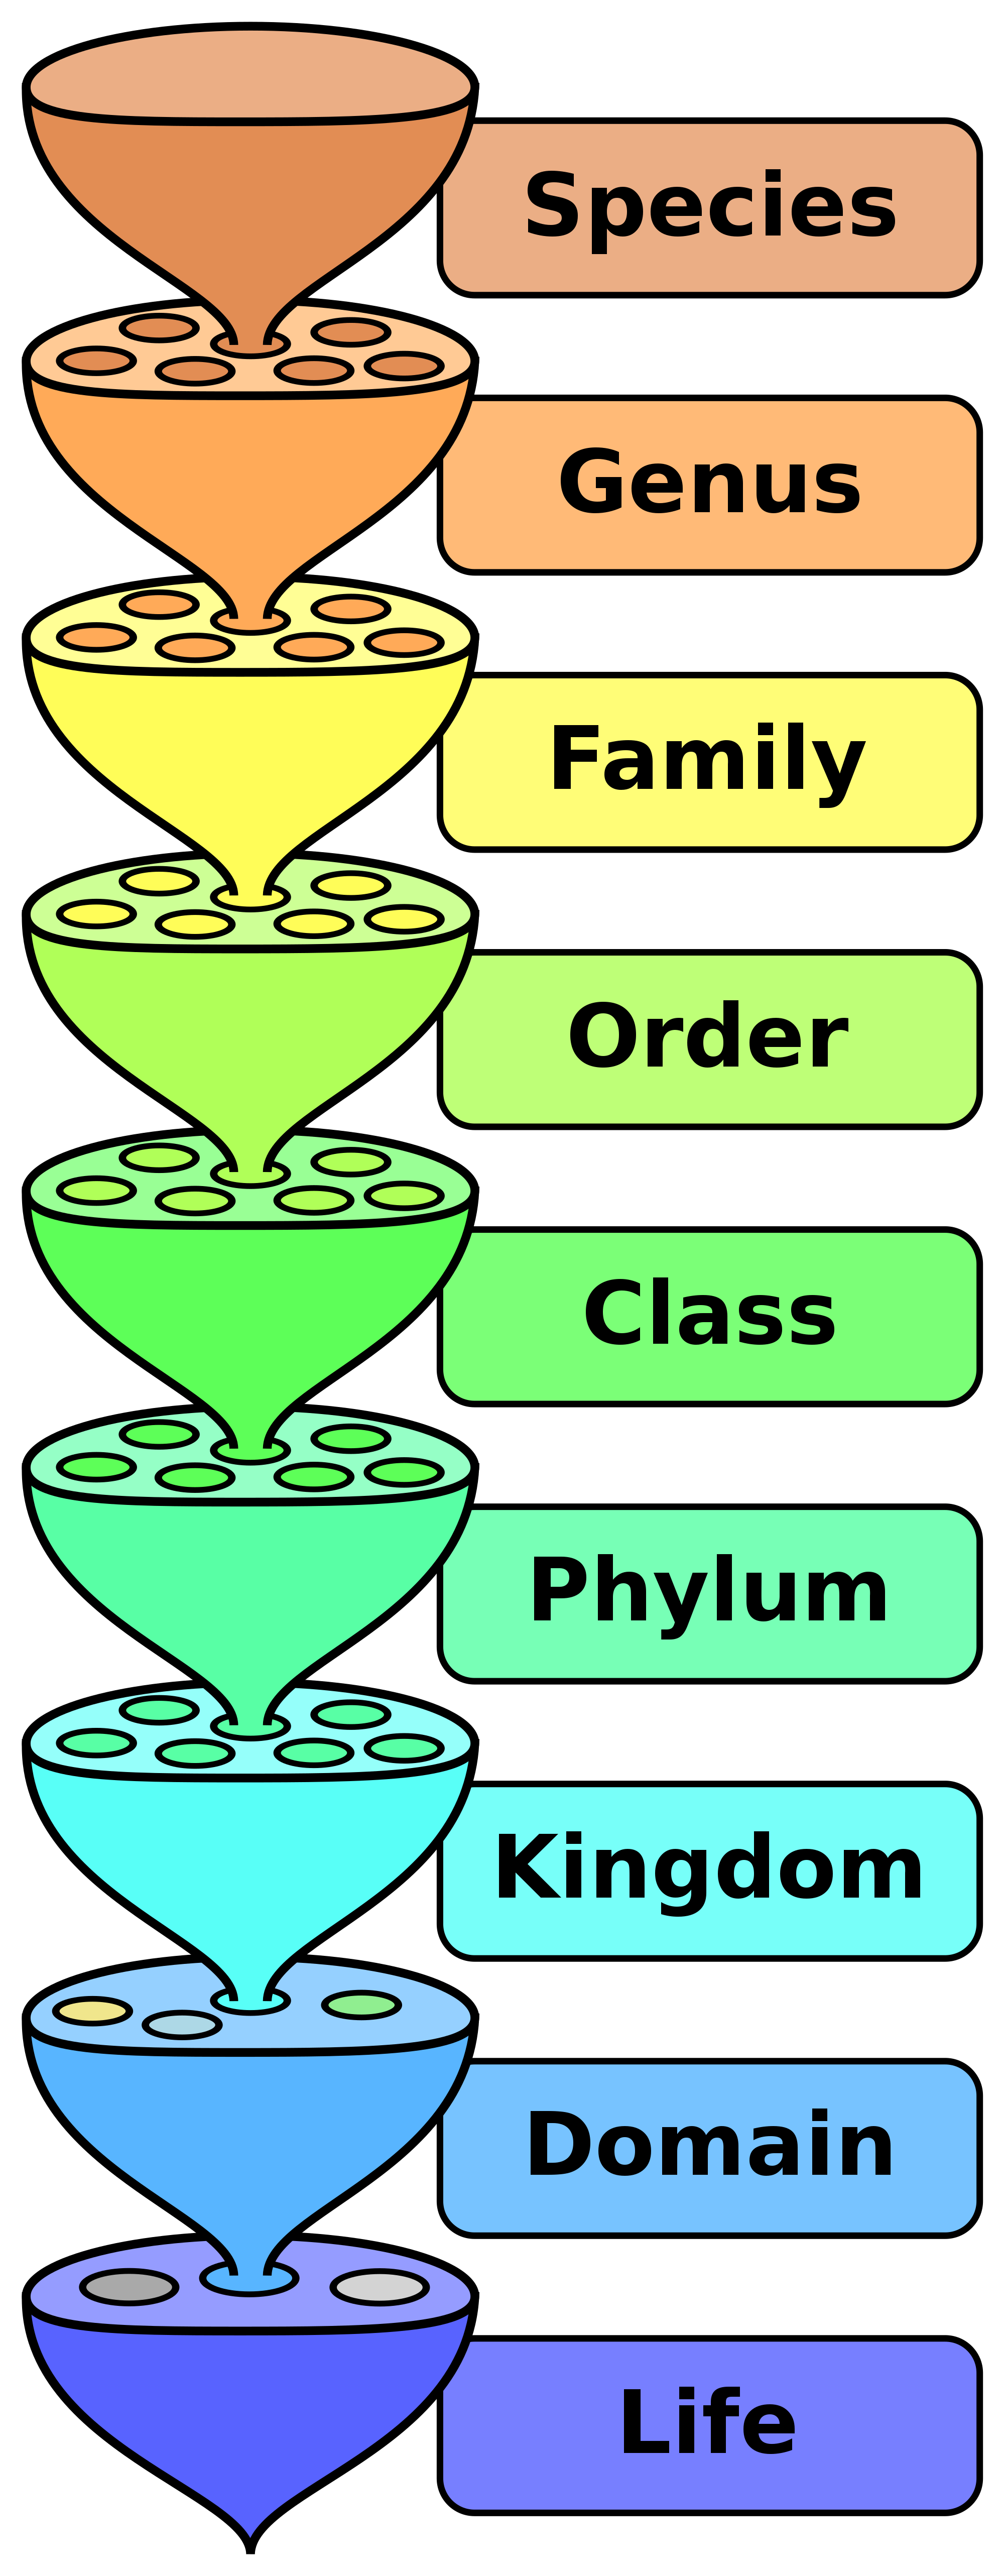
\includegraphics[width=0.7\linewidth]{./figures/life/Biological_classification_L_Pengo} 

}

\caption{\href{https://commons.wikimedia.org/wiki/File:Biological_classification_L_Pengo.svg}{The hierarchy of biological classification's eight major taxonomic ranks from the most specific (top) to the most general (bottom). Intermediate minor rankings are not shown. This diagram uses a 3 Domains / 6 Kingdoms format}}\label{fig:hierarchycartoon}
\end{figure}

Outside of these categories, there are obligate intracellular parasites that are ``on the edge of life'' in terms of metabolic activity, meaning that many scientists do not actually classify such structures as alive, due to their lack of at least one or more of the fundamental functions or characteristics that define life. They are classified as viruses, viroids, prions, or satellites.

The scientific name of an organism is generated from its genus and species. For example, humans are listed as Homo sapiens. Homo is the genus, and sapiens the species. When writing the scientific name of an organism, it is proper to capitalize the first letter in the genus and put all of the species in lowercase. Additionally, the entire term may be italicized or underlined.

The dominant classification system is called the \href{https://en.wikipedia.org/wiki/Linnaean_taxonomy}{Linnaean taxonomy}. It includes ranks and binomial nomenclature. How organisms are named is governed by international agreements such as the International Code of Nomenclature for algae, fungi, and plants (ICN), the International Code of Zoological Nomenclature (ICZN), and the International Code of Nomenclature of Bacteria (ICNB). The classification of viruses, viroids, prions, and all other sub-viral agents that demonstrate biological characteristics is conducted by the International Committee on Taxonomy of Viruses (ICTV) and is known as the International Code of Viral Classification and Nomenclature (ICVCN).

\href{https://en.wikipedia.org/wiki/Ecology}{Ecology} is the study of the distribution and abundance of living organisms, the interaction between them and their environment. An organism shares an environment that includes other organisms and biotic factors as well as local abiotic factors (non-living) such as climate and ecology. One reason that biological systems can be difficult to study is that so many different interactions with other organisms and the environment are possible, even on small scales. A microscopic bacterium responding to a local sugar gradient is responding to its environment as much as a lion searching for food in the African savanna. For any species, behaviors can be co-operative, competitive, parasitic, or symbiotic. Matters become more complex when two or more species interact in an ecosystem.

Ecological systems are studied at several different levels, from the scale of the ecology of individual organisms, to those of populations, to the ecosystems and finally the biosphere. The term population biology is often used interchangeably with population ecology, although population biology is more frequently used in the case of diseases, viruses, and microbes, while the term population ecology is more commonly applied to the study of plants and animals. Ecology draws on many subdisciplines.

\href{https://en.wikipedia.org/wiki/Ethology}{Ethology} is the study of animal behavior (particularly that of social animals such as primates and canids), and is sometimes considered a branch of zoology. Ethologists have been particularly concerned with the evolution of behavior and the understanding of behavior in terms of the theory of natural selection. In one sense, the first modern ethologist was Charles Darwin, whose book, The Expression of the Emotions in Man and Animals, influenced many ethologists to come.



\begin{figure}

{\centering 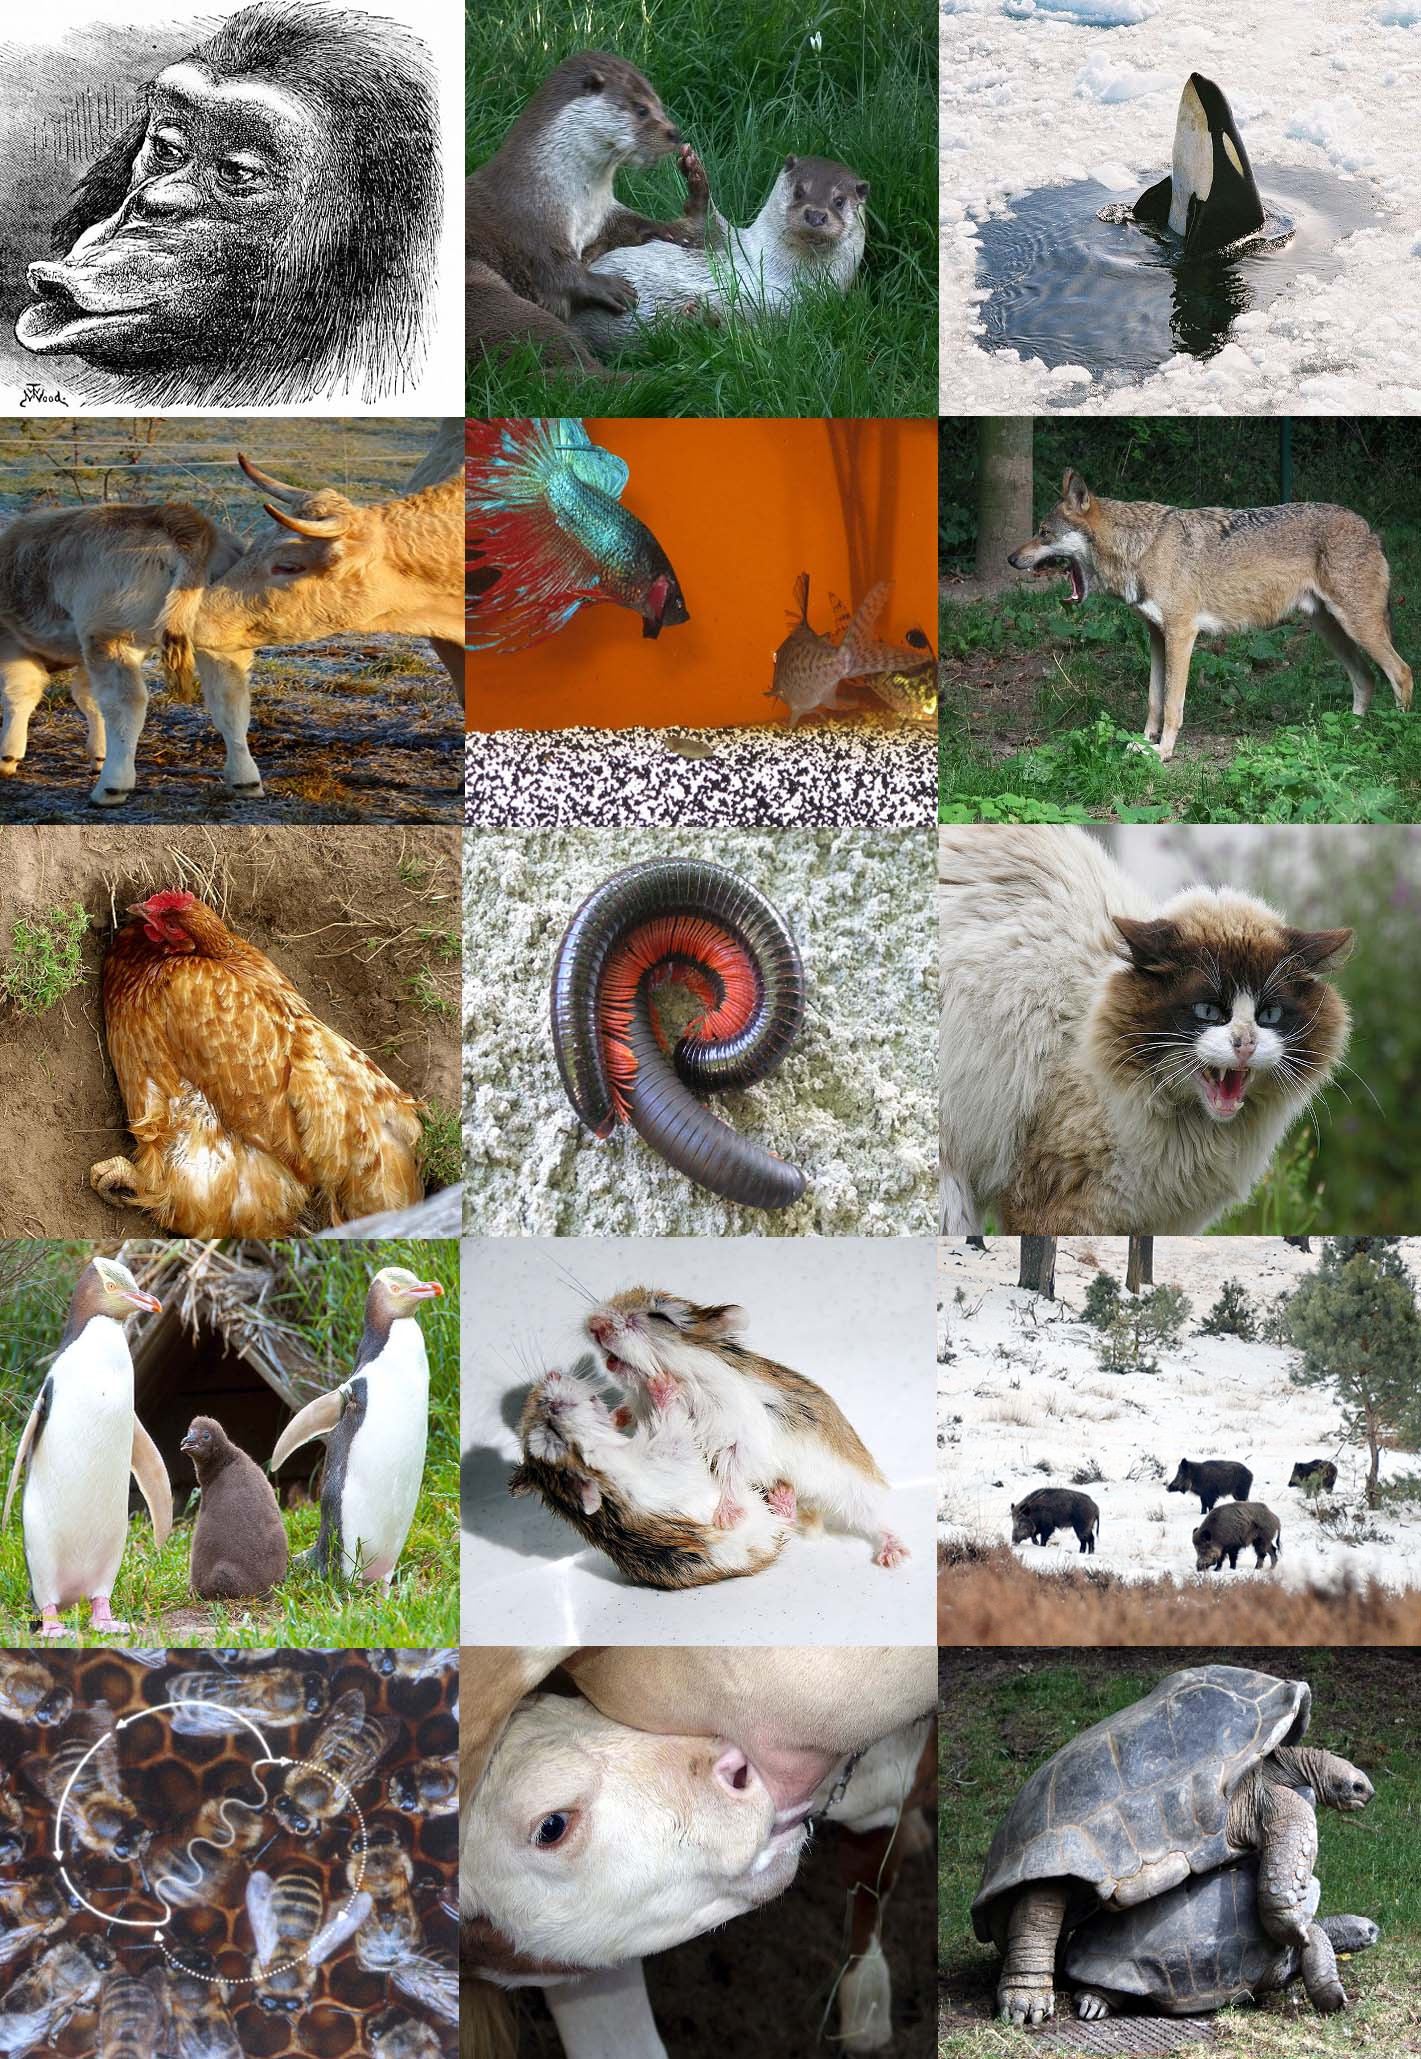
\includegraphics[width=0.7\linewidth]{./figures/life/Ethology_diversity_2} 

}

\caption{\href{https://commons.wikimedia.org/wiki/File:Ethology_diversity_2.jpg}{A range of animal behaviours.}}\label{fig:ethology}
\end{figure}

Biogeography studies the spatial distribution of organisms on the Earth, focusing on such topics as plate tectonics, climate change, dispersal and migration, and cladistics.

\hypertarget{science}{%
\section{Science}\label{science}}

\href{https://en.wikipedia.org/wiki/Science}{Science} (from the Latin word scientia, meaning ``knowledge'') is a systematic enterprise that builds and organizes knowledge in the form of testable explanations and predictions about the universe.

Scientists are individuals who conduct scientific research to advance knowledge in an area of interest. In classical antiquity, there was no real ancient analog of a modern scientist. Instead, philosophers engaged in the philosophical study of nature called natural philosophy, a precursor of natural science. It was not until the 19th century that the term scientist came into regular use after it was coined by the theologian, philosopher, and historian of science William Whewell in 1833. In modern times, many professional scientists are trained in an academic setting and upon completion, attain an academic degree, with the highest degree being a doctorate such as a Doctor of Philosophy (PhD). Many scientists pursue careers in various sectors of the economy such as academia, industry, government, and nonprofit organizations.



\begin{figure}

{\centering 
\includegraphics[width=0.7\linewidth]{./figures/life/Researcher_looking_through_microscope} 

}

\caption{\href{https://commons.wikimedia.org/wiki/File:Researcher_looking_through_microscope.jpg}{Two scientists working at the National Cancer Institute which is part of the National Institutes of Health of the United States of America.}}\label{fig:twoscientists}
\end{figure}

The roles of ``scientists'', and their predecessors before the emergence of modern scientific disciplines, have evolved considerably over time. Scientists of different eras (and before them, natural philosophers and others who contributed to the development of science) have had widely different places in society, and the social norms, ethical values, and epistemic virtues associated with scientists---and expected of them---have changed over time as well.

Some historians point to the Scientific Revolution that began in 16th century as the period when science in a recognizably modern form developed. It wasn't until the 19th century that sufficient socioeconomic changes occurred for scientists to emerge as a major profession.

The presence of women in science spans the earliest times of the history of science wherein they have made significant contributions. Historians with an interest in gender and science have researched the scientific endeavors and accomplishments of women, the barriers they have faced, and the strategies implemented to have their work peer-reviewed and accepted in major scientific journals and other publications.

The involvement of women in the field of medicine occurred in several early civilizations, and the study of natural philosophy in ancient Greece was open to women. Women contributed to the proto-science of alchemy in the first or second centuries AD. During the Middle Ages, religious convents were an important place of education for women, and some of these communities provided opportunities for women to contribute to scholarly research. The 11th century saw the emergence of the first universities; women were, for the most part, excluded from university education. Outside academia, botany was the science that benefitted most from contributions of women in early modern times. Gender roles were largely deterministic in the eighteenth century and women made substantial advances in science. During the nineteenth century, women were excluded from most formal scientific education, but they began to be admitted into learned societies during this period. In the later nineteenth century, the rise of the women's college provided jobs for women scientists and opportunities for education. \href{https://en.wikipedia.org/wiki/Marie_Curie}{Marie Curie}, a physicist and chemist who conducted pioneering research on radioactive decay, was the first woman to receive a Nobel Prize in Physics and became the first person to receive a second Nobel Prize in Chemistry. Forty women have been awarded the Nobel Prize between 1901 and 2010. Seventeen women have been awarded the Nobel Prize in physics, chemistry, physiology or medicine.



\begin{figure}

{\centering 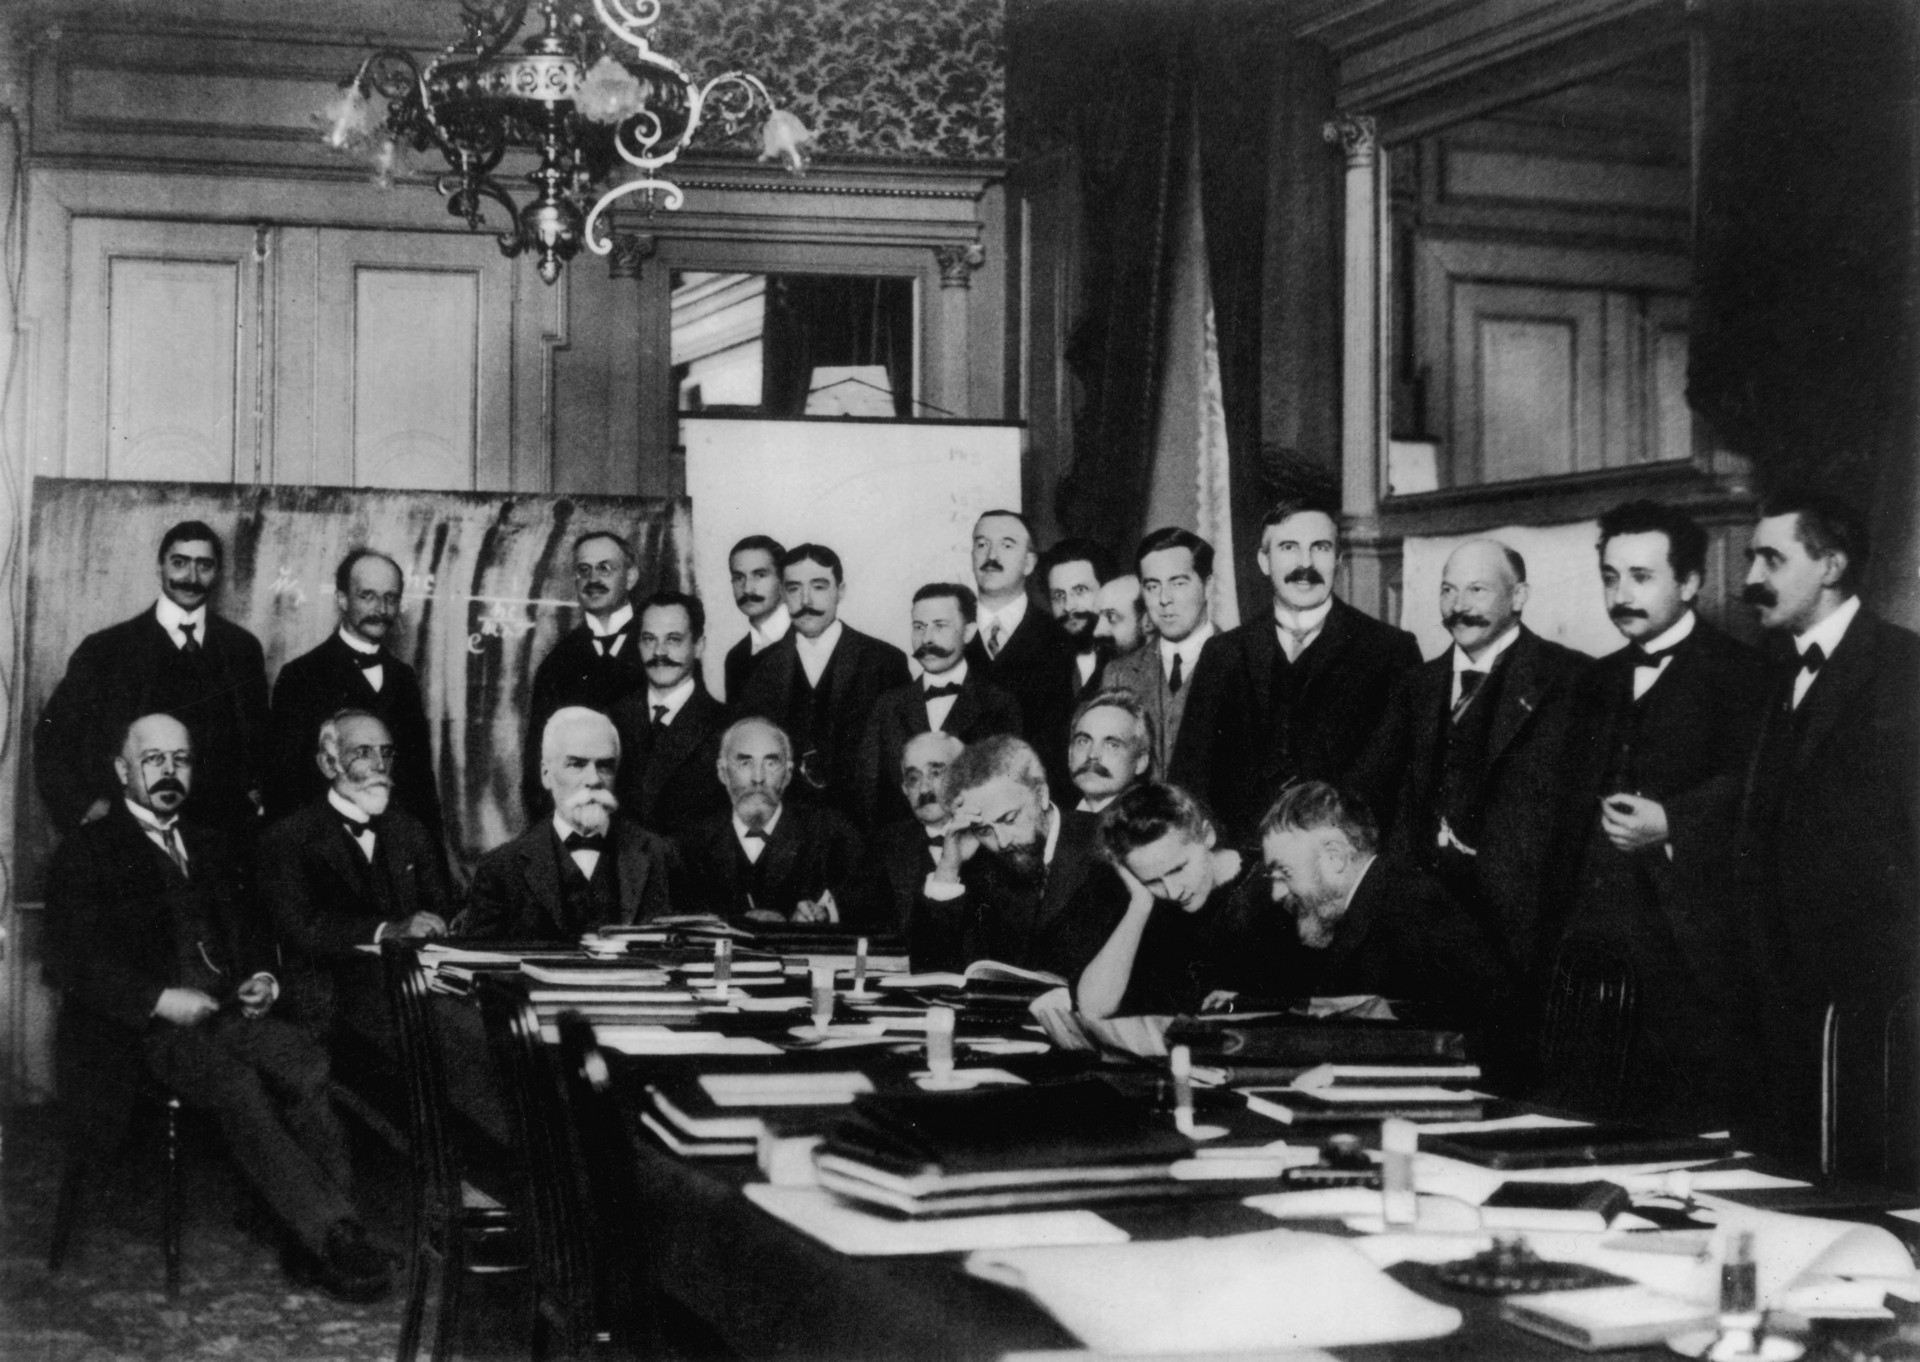
\includegraphics[width=0.7\linewidth]{./figures/life/1911_Solvay_conference} 

}

\caption{\href{https://commons.wikimedia.org/wiki/File:1911_Solvay_conference.jpg}{At First Solvay Conference (1911), Marie Curie (seated, second from right) confers with Henri Poincaré; standing, fourth from right, is Rutherford; second from right, Einstein; far right, Paul Langevin}}\label{fig:mariecuriesolvay}
\end{figure}

\href{https://en.wikipedia.org/wiki/List_of_African-American_inventors_and_scientists}{A list of African Americans inventors and scientists} documents many of the African-Americans who have invented a multitude of items or made discoveries in the course of their lives. These have ranged from practical everyday devices to applications and scientific discoveries in diverse fields, including physics, biology, math, plus the medical, nuclear and space science.



\begin{figure}

{\centering \includegraphics[width=0.7\linewidth]{./figures/life/George_Washington_Carver_c1910_-_Restoration} 

}

\caption{\href{https://en.wikipedia.org/wiki/George_Washington_Carver}{George Washington Carver} (1860s -- January 5, 1943) was an American agricultural scientist and inventor who promoted alternative crops to cotton and methods to prevent soil depletion. He was the most prominent black scientist of the early 20th century. Apart from his work to improve the lives of farmers, Carver was also a leader in promoting environmentalism. He received numerous honors for his work, including the Spingarn Medal of the NAACP. In an era of high racial polarization, his fame reached beyond the black community. He was widely recognized and praised in the white community for his many achievements and talents. In 1941, Time magazine dubbed Carver a ``Black Leonardo''.}\label{fig:gwcarter}
\end{figure}

Scientists exhibit a strong curiosity about reality, with some scientists having a desire to apply scientific knowledge for the benefit of health, nations, environment, or industries. Other motivations include recognition by their peers and prestige. The Nobel Prize, a widely regarded prestigious award, is awarded annually to those who have achieved scientific advances in the fields of medicine, physics, chemistry, and economics.

The earliest roots of science can be traced to Ancient Egypt and Mesopotamia in around 3500 to 3000 BCE. Their contributions to mathematics, astronomy, and medicine entered and shaped Greek natural philosophy of classical antiquity, whereby formal attempts were made to provide explanations of events in the physical world based on natural causes. After the fall of the Western Roman Empire, knowledge of Greek conceptions of the world deteriorated in Western Europe during the early centuries (400 to 1000 CE) of the Middle Ages but was preserved in the Muslim world during the Islamic Golden Age. The recovery and assimilation of Greek works and Islamic inquiries into Western Europe from the 10th to 13th century revived ``natural philosophy'', which was later transformed by the Scientific Revolution that began in the 16th century as new ideas and discoveries departed from previous Greek conceptions and traditions. The scientific method soon played a greater role in knowledge creation and it was not until the 19th century that many of the institutional and professional features of science began to take shape; along with the changing of ``natural philosophy'' to ``natural science.''

Modern science is typically divided into three major branches that consist of the natural sciences (e.g., biology, chemistry, and physics), which study nature in the broadest sense; the social sciences (e.g., economics, psychology, and sociology), which study individuals and societies; and the formal sciences (e.g., logic, mathematics, and theoretical computer science), which study abstract concepts. There is disagreement, however, on whether the formal sciences actually constitute a science as they do not rely on empirical evidence. Disciplines that use existing scientific knowledge for practical purposes, such as engineering and medicine, are described as applied sciences.

Science is based on research, which is commonly conducted in academic and research institutions as well as in government agencies and companies. The practical impact of scientific research has led to the emergence of science policies that seek to influence the scientific enterprise by prioritizing the development of commercial products, armaments, health care, and environmental protection.

Natural science is concerned with the description, prediction, and understanding of natural phenomena based on empirical evidence from observation and experimentation.

\hypertarget{scientific-terminology}{%
\subsection{Scientific Terminology}\label{scientific-terminology}}

\href{https://en.wikipedia.org/wiki/Scientific_terminology}{Scientific terminology} is the part of the language that is used by scientists in the context of their professional activities. While studying nature, scientists often encounter or create new material or immaterial objects and concepts and are compelled to name them.

In modern science and its applied fields such as technology and medicine, a knowledge of classical languages is not as rigid a prerequisite as it used to be. However, traces of their influence remain. Firstly, languages such as Greek, Latin and Arabic -- either directly or via more recently derived languages such as French -- have provided not only most of the technical terms used in Western science, but also a de facto vocabulary of roots, prefixes and suffixes for the construction of new terms as required. Echoes of the consequences sound in remarks such as "Television? The word is half Latin and half Greek.

Branches of science that are based, however tenuously, on fields of study known to the ancients, or that were established by more recent workers familiar with Greek and Latin, often use terminology that is fairly correct descriptive Latin, or occasionally Greek. Descriptive human anatomy or works on biological morphology often use such terms, for example, musculus gluteus maximus simply means the ``largest rump muscle'', where musculus was the Latin for ``little mouse'' and the name applied to muscles. During the last two centuries there has been an increasing tendency to modernise the terminology, though how beneficial that might be is subject to discussion. In other descriptive anatomical terms, whether in vertebrates or invertebrates, a frenum (a structure for keeping something in place) is simply the Latin for a bridle; and a foramen (a passage or perforation) also is the actual Latin word.

A special class of terminology that overwhelmingly is derived from classical sources, is biological classification, in which binomial nomenclature still is most often based on classical origins. \href{https://en.wikipedia.org/wiki/Binomial_nomenclature}{Binomial nomenclature} (``two-term naming system'') or binary nomenclature, is a formal system of naming species of living things by giving each a name composed of two parts, both of which use Latin grammatical forms, although they can be based on words from other languages. Such a name is called a binomial name (which may be shortened to just ``binomial''), a binomen, binominal name or a scientific name; more informally it is also called a Latin name.

The first part of the name -- the generic name -- identifies the genus to which the species belongs, while the second part -- the specific name or specific epithet -- identifies the species within the genus. For example, humans belong to the genus Homo and within this genus to the species \emph{Homo sapiens}. \emph{Tyrannosaurus rex} is probably the most widely known binomial. The formal introduction of this system of naming species is credited to \href{https://en.wikipedia.org/wiki/Carl_Linnaeus}{Carl Linnaeus}, effectively beginning with his work Species Plantarum in 1753. But \href{https://en.wikipedia.org/wiki/Gaspard_Bauhin}{Gaspard Bauhin}, in as early as 1622, had introduced in his book Pinax theatri botanici (English, Illustrated exposition of plants) many names of genera that were later adopted by Linnaeus.

The application of binomial nomenclature is now governed by various internationally agreed codes of rules, of which the two most important are the International Code of Zoological Nomenclature (ICZN) for animals and the International Code of Nomenclature for algae, fungi, and plants (ICNafp).

In modern usage, the first letter of the first part of the name, the genus, is always capitalized in writing, while that of the second part is not, even when derived from a proper noun such as the name of a person or place. Similarly, both parts are italicized when a binomial name occurs in normal text (or underlined in handwriting). Thus the binomial name of the annual phlox (named after botanist Thomas Drummond) is now written as \href{https://en.wikipedia.org/wiki/Phlox_drummondii}{\emph{Phlox drummondii}}.

\hypertarget{the-scientific-method}{%
\subsection{The Scientific Method}\label{the-scientific-method}}

The \href{https://en.wikipedia.org/wiki/Scientific_method}{scientific method} is the process by which science is carried out. Scientific research involves using the scientific method, which seeks to objectively explain the events of nature in a reproducible way. An explanatory thought experiment or hypothesis is put forward as explanation using principles such as parsimony (also known as ``Occam's Razor'') and are generally expected to seek consilience -- fitting well with other accepted facts related to the phenomena.

A \href{https://en.wikipedia.org/wiki/Hypothesis}{hypothesis} (plural hypotheses) is a proposed explanation for a phenomenon. For a hypothesis to be a scientific hypothesis, the scientific method requires that one can test it. An experiment is a procedure carried out to support, refute, or validate a hypothesis. Experiments provide insight into cause-and-effect by demonstrating what outcome occurs when a particular factor is manipulated. Experiments vary greatly in goal and scale, but always rely on repeatable procedure and logical analysis of the results. Scientists generally base scientific hypotheses on previous observations that cannot satisfactorily be explained with the available scientific theories. Even though the words ``hypothesis'' and ``theory'' are often used synonymously, a scientific hypothesis is not the same as a scientific theory. A working hypothesis is a provisionally accepted hypothesis proposed for further research, in a process beginning with an educated guess or thought.

\href{https://en.wikipedia.org/wiki/Occam\%27s_razor}{Occam's razor} or law of parsimony (Latin: lex parsimoniae) is the problem-solving principle that ``entities should not be multiplied without necessity.'' The idea is attributed to English Franciscan friar William of Ockham (c.~1287--1347), a scholastic philosopher and theologian who used a preference for simplicity to defend the idea of divine miracles. It is variously paraphrased by statements like ``the simplest explanation is most likely the right one''. This philosophical razor advocates that when presented with competing hypotheses about the same prediction, one should select the solution with the fewest assumptions, and that this is not meant to be a way of choosing between hypotheses that make different predictions.

A hypothesis is used to make falsifiable predictions that are testable by experiment or observation. The predictions are to be posted before a confirming experiment or observation is sought, as proof that no tampering has occurred. Disproof of a prediction is evidence of progress. This is done partly through observation of natural phenomena, but also through experimentation that tries to simulate natural events under controlled conditions as appropriate to the discipline (in the observational sciences, such as astronomy or geology, a predicted observation might take the place of a controlled experiment). Experimentation is especially important in science to help establish causal relationships (to avoid the correlation fallacy).

\href{https://en.wikipedia.org/wiki/Falsifiability}{Falsifiability} or refutability is the capacity for a statement, theory or hypothesis to be contradicted by evidence. For example, the statement ``All swans are white'' is falsifiable because one can observe that black swans exist

When a hypothesis proves unsatisfactory, it is either modified or discarded. If the hypothesis survived testing, it may become adopted into the framework of a scientific theory, a logically reasoned, self-consistent model or framework for describing the behavior of certain natural phenomena. A theory typically describes the behavior of much broader sets of phenomena than a hypothesis; commonly, a large number of hypotheses can be logically bound together by a single theory. Thus a theory is a hypothesis explaining various other hypotheses. In that vein, theories are formulated according to most of the same scientific principles as hypotheses. In addition to testing hypotheses, scientists may also generate a model, an attempt to describe or depict the phenomenon in terms of a logical, physical or mathematical representation and to generate new hypotheses that can be tested, based on observable phenomena.

While performing experiments to test hypotheses, scientists may have a preference for one outcome over another, and so it is important to ensure that science as a whole can eliminate this bias. This can be achieved by careful experimental design, transparency, and a thorough peer review process of the experimental results as well as any conclusions. After the results of an experiment are announced or published, it is normal practice for independent researchers to double-check how the research was performed, and to follow up by performing similar experiments to determine how dependable the results might be. Taken in its entirety, the scientific method allows for highly creative problem solving while minimizing any effects of subjective bias on the part of its users (especially the confirmation bias).

\hypertarget{dissemination-of-scientific-knowledge}{%
\subsection{Dissemination of Scientific Knowledge}\label{dissemination-of-scientific-knowledge}}

Scientific research is published in an enormous range of scientific literature. Scientific journals communicate and document the results of research carried out in universities and various other research institutions, serving as an archival record of science. The first scientific journals, Journal des Sçavans followed by the Philosophical Transactions, began publication in 1665. Since that time the total number of active periodicals has steadily increased. In 1981, one estimate for the number of scientific and technical journals in publication was 11,500. The United States National Library of Medicine currently indexes 5,516 journals that contain articles on topics related to the life sciences. Although the journals are in 39 languages, 91 percent of the indexed articles are published in English.

Most scientific journals cover a single scientific field and publish the research within that field; the research is normally expressed in the form of a scientific paper. Science has become so pervasive in modern societies that it is generally considered necessary to communicate the achievements, news, and ambitions of scientists to a wider populace.

An important aspect of the dissemination of scientific results is scholarly \href{https://en.wikipedia.org/wiki/Peer_review}{peer review} (also known as refereeing). This is the process of subjecting an author's scholarly work, research, or ideas to the scrutiny of others who are experts in the same field, before a paper describing this work is published in a journal, conference proceedings or as a book. The peer review helps the publisher (that is, the editor-in-chief, the editorial board or the program committee) decide whether the work should be accepted, considered acceptable with revisions, or rejected.

Researchers have peer reviewed manuscripts prior to publishing them in a variety of ways since the 18th century. The main goal of this practice is to improve the relevance and accuracy of scientific discussions. Even though experts often criticize peer review for a number of reasons, the process is still often considered the ``gold standard'' of science. Occasionally however, peer review approves studies that are later found to be wrong and rarely deceptive or fraudulent results are discovered prior to publication. Thus, there seems to be an element of discord between the ideology behind and the practice of peer review. By failing to effectively communicate that peer review is imperfect, the message conveyed to the wider public is that studies published in peer-reviewed journals are ``true'' and that peer review protects the literature from flawed science.

Open access (OA) is a set of principles and a range of practices through which research outputs are distributed online, free of cost or other access barriers. With open access strictly defined (according to the 2001 definition), or libre open access, barriers to copying or reuse are also reduced or removed by applying an open license for copyright.

The main focus of the open access movement is ``peer reviewed research literature.'' Historically, this has centered mainly on print-based academic journals. Whereas conventional (non-open access) journals cover publishing costs through access tolls such as subscriptions, site licenses or pay-per-view charges, open-access journals are characterised by funding models which do not require the reader to pay to read the journal's contents but the authors may be charged for the cost of publishing .

\hypertarget{philosophy-of-science}{%
\section{Philosophy of Science}\label{philosophy-of-science}}

\href{https://en.wikipedia.org/wiki/Philosophy_of_science}{Philosophy of science} is a branch of philosophy concerned with the foundations, methods, and implications of science. The central questions of this study concern what qualifies as science, the reliability of scientific theories, and the ultimate purpose of science.

There is no consensus among philosophers about many of the central problems concerned with the philosophy of science, including whether science can reveal the truth about unobservable things and whether scientific reasoning can be justified at all.

Problems of philosophy of science include

\begin{itemize}
\tightlist
\item
  defining science
\item
  scientific explanation
\item
  justifying science
\item
  separability of theory and obsrvation
\item
  purpose of science
\item
  values and science
\end{itemize}

Scientists usually take for granted a set of basic assumptions that are needed to justify the scientific method: (1) that there is an objective reality shared by all rational observers; (2) that this objective reality is governed by natural laws; (3) that these laws can be discovered by means of systematic observation and experimentation. Philosophy of science seeks a deep understanding of what these underlying assumptions mean and whether they are valid.

The belief that scientific theories should and do represent metaphysical reality is known as realism. It can be contrasted with anti-realism, the view that the success of science does not depend on it being accurate about unobservable entities such as electrons. One form of anti-realism is idealism, the belief that the mind or consciousness is the most basic essence, and that each mind generates its own reality. In an idealistic world view, what is true for one mind need not be true for other minds.

There are different schools of thought in philosophy of science. The most popular position is empiricism, which holds that knowledge is created by a process involving observation and that scientific theories are the result of generalizations from such observations. Empiricism generally encompasses inductivism, a position that tries to explain the way general theories can be justified by the finite number of observations humans can make and hence the finite amount of empirical evidence available to confirm scientific theories. This is necessary because the number of predictions those theories make is infinite, which means that they cannot be known from the finite amount of evidence using deductive logic only. Many versions of empiricism exist, with the predominant ones being Bayesianism and the hypothetico-deductive method.

Logical positivism, later called logical empiricism, and both of which together are also known as neopositivism, is a branch in Western philosophy whose central thesis is the verification principle (also known as the verifiability criterion of meaning). This theory of knowledge asserts that only statements verifiable through direct observation or logical proof are meaningful. Starting in the late 1920s, groups of philosophers, scientists, and mathematicians formed the Berlin Circle and the Vienna Circle, which, in these two cities, would propound the ideas of logical positivism.

Flourishing in several European centres through the 1930s, the movement sought to prevent confusion rooted in unclear language and unverifiable claims by converting philosophy into ``scientific philosophy'', which, according to the logical positivists, ought to share the bases and structures of empirical sciences' best examples, such as Albert Einstein's general theory of relativity. Despite its ambition to overhaul philosophy by studying and mimicking the extant conduct of empirical science, logical positivism became erroneously stereotyped as a movement to regulate the scientific process and to place strict standards on it.

After World War II, the movement shifted to a milder variant, logical empiricism, led mainly by \href{https://en.wikipedia.org/wiki/Carl_Gustav_Hempel}{Carl Hempel}, who, during the rise of Nazism, had immigrated to the United States. In the ensuing years, the movement's central premises, still unresolved, were criticised by other philosophers, particularly \href{https://en.wikipedia.org/wiki/Willard_Van_Orman_Quine}{Willard van Orman Quine} and by Austrian-British philosopher \href{https://en.wikipedia.org/wiki/Karl_Popper}{Karl Popper}.

Empiricism has stood in contrast to rationalism, the position originally associated with Descartes, which holds that knowledge is created by the human intellect, not by observation. Critical rationalism is a contrasting 20th-century approach to science, first defined Karl Popper. Popper rejected the way that empiricism describes the connection between theory and observation. He claimed that theories are not generated by observation, but that observation is made in the light of theories and that the only way a theory can be affected by observation is when it comes in conflict with it. Popper proposed replacing verifiability with falsifiability as the landmark of scientific theories and replacing induction with falsification as the empirical method. Popper further claimed that there is actually only one universal method, not specific to science: the negative method of criticism, trial and error. It covers all products of the human mind, including science, mathematics, philosophy, and art.

Another approach, instrumentalism, colloquially termed ``\href{https://physicstoday.scitation.org/doi/10.1063/1.1768652}{shut up and calculate},'' emphasizes the utility of theories as instruments for explaining and predicting phenomena. It views scientific theories as black boxes with only their input (initial conditions) and output (predictions) being relevant. Consequences, theoretical entities, and logical structure are claimed to be something that should simply be ignored and that scientists should not make a fuss about (see interpretations of quantum mechanics). Close to instrumentalism is constructive empiricism, according to which the main criterion for the success of a scientific theory is whether what it says about observable entities is true.

In his book The \href{https://en.wikipedia.org/wiki/The_Structure_of_Scientific_Revolutions}{Structure of Scientific Revolutions} the American philosopher of science \href{https://en.wikipedia.org/wiki/Thomas_Kuhn}{Thomas Samuel Kuhn} made several claims concerning the progress of scientific knowledge: that scientific fields undergo periodic ``paradigm shifts'' rather than solely progressing in a linear and continuous way, and that these paradigm shifts open up new approaches to understanding what scientists would never have considered valid before; and that the notion of scientific truth, at any given moment, cannot be established solely by objective criteria but is defined by a consensus of a scientific community. Competing paradigms are frequently incommensurable; that is, they are competing and irreconcilable accounts of reality. Thus, our comprehension of science can never rely wholly upon ``objectivity'' alone. Science must account for subjective perspectives as well, since all objective conclusions are ultimately founded upon the subjective conditioning/worldview of its researchers and participants.

A scientific theory is empirical and is always open to falsification if new evidence is presented. That is, no theory is ever considered strictly certain as science accepts the concept of fallibilism. The philosopher of science Karl Popper sharply distinguished truth from certainty. He wrote that scientific knowledge ``consists in the search for truth,'' but it "is not the search for certainty \ldots{} All human knowledge is fallible and therefore uncertain.

New scientific knowledge rarely results in vast changes in our understanding. Knowledge in science is gained by a gradual synthesis of information from different experiments by various researchers across different branches of science; it is more like a climb than a leap. Theories vary in the extent to which they have been tested and verified, as well as their acceptance in the scientific community. For example, heliocentric theory, the theory of evolution, relativity theory, and germ theory still bear the name ``theory'' even though, in practice, they are considered factual. Philosopher Barry Stroud adds that, although the best definition for ``knowledge'' is contested, being skeptical and entertaining the possibility that one is incorrect is compatible with being correct. Therefore, scientists adhering to proper scientific approaches will doubt themselves even once they possess the truth.

The Polish and Israeli physician, biologist and philosopher of science \href{https://en.wikipedia.org/wiki/Ludwik_Fleck}{Ludwik Fleck} wrote in his 1935 book ``Entstehung und Entwicklung einer wissenschaftlichen Tatsache; Einführung in die Lehre vom Denkstil und Denkkollektiv'' that the development of truth in scientific research was an unattainable ideal as different researchers were locked into thought collectives (or thought-styles). This means ``that a pure and direct observation cannot exist: in the act of perceiving objects the observer, i.e.~the epistemological subject, is always influenced by the epoch and the environment to which he belongs, that is by what Fleck calls the thought style.'' A ``truth'' was a relative value, expressed in the language or symbolism of the thought collective in which it belonged, and subject to the social and temporal structure of this collective. To state therefore that a specific truth is true or false is impossible. It is true in its own collective, but incomprehensible or unverifiable in most others. He felt that the development of scientific insights was not unidirectional and does not consist of just accumulating new pieces of information, but also in overthrowing the old ones. This overthrowing of old insights is difficult because a collective attains over time a specific way of investigating, bringing with it a blindness to alternative ways of observing and conceptualization. Change was especially possible when members of two thought collectives met and cooperated in observing, formulating hypothesis and ideas. He strongly advocated comparative epistemology. This approach anticipated later developments in social constructionism, and especially the development of critical science and technology studies.

In his book Against Method and Science in a Free Society the philosopher \href{https://en.wikipedia.org/wiki/Paul_Feyerabend}{Paul Feyerabend} defended the idea that there are no methodological rules which are always used by scientists. He objected to any single prescriptive scientific method on the grounds that any such method would limit the activities of scientists, and hence restrict scientific progress. In his view, science would benefit most from a ``dose'' of theoretical anarchism. He also thought that theoretical anarchism was desirable because it was more humanitarian than other systems of organization, by not imposing rigid rules on scientists.

\begin{quote}
For is it not possible that science as we know it today, or a ``search for the truth'' in the style of traditional philosophy, will create a monster? Is it not possible that an objective approach that frowns upon personal connections between the entities examined will harm people, turn them into miserable, unfriendly, self-righteous mechanisms without charm or humour? ``Is it not possible,'' asks Kierkegaard, ``that my activity as an objective {[}or critico-rational{]} observer of nature will weaken my strength as a human being?'' I suspect the answer to many of these questions is affirmative and I believe that a reform of the sciences that makes them more anarchic and more subjective (in Kierkegaard's sense) is urgently needed.
\end{quote}

\begin{quote}
Against Method: Outline of an Anarchistic Theory of Knowledge (1975)
\end{quote}

Feyerabend's position was seen as radical in the philosophy of science, because it implies that philosophy can neither succeed in providing a general description of science, nor in devising a method for differentiating products of science from non-scientific entities like myths. (Feyerabend's position also implies that philosophical guidelines should be ignored by scientists, if they are to aim for progress.)

To support his position that methodological rules generally do not contribute to scientific success, Feyerabend provides counterexamples to the claim that (good) science operates according to a certain fixed method. He took some examples of episodes in science that are generally regarded as indisputable instances of progress (e.g.~the Copernican revolution), and argued that these episodes violated all common prescriptive rules of science. Moreover, he claimed that applying such rules in these historical situations would actually have prevented scientific revolution.

According to Feyerabend, new theories came to be accepted not because of their accord with scientific method, but because their supporters made use of any trick -- rational, rhetorical or ribald -- in order to advance their cause. Without a fixed ideology, or the introduction of religious tendencies, the only approach which does not inhibit progress (using whichever definition one sees fit) is ``anything goes'': ``\,`anything goes' is not a `principle' I hold\ldots{} but the terrified exclamation of a rationalist who takes a closer look at history.''

\hypertarget{science-and-religion}{%
\section{Science And Religion}\label{science-and-religion}}

Historians of \href{https://en.wikipedia.org/wiki/Relationship_between_religion_and_science}{science and of religion}, philosophers, theologians, scientists, and others from various geographical regions and cultures have addressed numerous aspects of the relationship between religion and science. Critical questions in this debate include whether religion and science are compatible, whether religious beliefs can be conducive to science (or necessarily inhibit it), and what the nature of religious beliefs is. Another question is whether or not science has for some people become a new religion.

Even though the ancient and medieval worlds did not have conceptions resembling the modern understandings of ``science'' or of ``religion'', certain elements of modern ideas on the subject recur throughout history. The pair-structured phrases ``religion and science'' and ``science and religion'' first emerged in the literature in the 19th century. This coincided with the refining of ``science'' (from the studies of ``natural philosophy'') and of ``religion'' as distinct concepts in the preceding few centuries---partly due to professionalization of the sciences, the Protestant Reformation, colonization, and globalization. Since then the relationship between science and religion has been characterized in terms of `conflict', `harmony', `complexity', and `mutual independence', among others.

Both science and religion are complex social and cultural endeavors that vary across cultures and change over time. Most scientific (and technical) innovations prior to the scientific revolution were achieved by societies organized by religious traditions. Ancient pagan, Islamic, and Christian scholars pioneered individual elements of the scientific method. Roger Bacon, often credited with formalizing the scientific method, was a Franciscan friar. Confucian thought, whether religious or non-religious in nature, has held different views of science over time. Many 21st-century Buddhists view science as complementary to their beliefs. While the classification of the material world by the ancient Indians and Greeks into air, earth, fire and water was more metaphysical, and figures like Anaxagoras questioned certain popular views of Greek divinities, medieval Middle Eastern scholars empirically classified materials.

Events in Europe such as the Galileo affair of the early 17th century, associated with the scientific revolution and the Age of Enlightenment, led scholars such as John William Draper to postulate (c.  1874) a conflict thesis, suggesting that religion and science have been in conflict methodologically, factually and politically throughout history. Some contemporary scientists (such as Richard Dawkins, Lawrence Krauss, Peter Atkins, and Donald Prothero) subscribe to this thesis. However, the conflict thesis has lost favor among most contemporary historians of science.

Many scientists, philosophers, and theologians throughout history, such as Francisco Ayala, Kenneth R. Miller and Francis Collins, have seen compatibility or interdependence between religion and science. Biologist Stephen Jay Gould, other scientists, and some contemporary theologians regard religion and science as non-overlapping magisteria, addressing fundamentally separate forms of knowledge and aspects of life. Some theologians or historians of science, including John Lennox, Thomas Berry, Brian Swimme and Ken Wilber propose an interconnection between science and religion, while others such as Ian Barbour believe there are even parallels.

Public acceptance of scientific facts may sometimes be influenced by religious beliefs such as in the United States, where some reject the concept of evolution by natural selection, especially regarding human beings. Nevertheless, the American National Academy of Sciences has written that ``the evidence for evolution can be fully compatible with religious faith'', a view endorsed by many religious denominations.

The concepts of ``science'' and ``religion'' are a recent invention: ``religion'' emerged in the 17th century in the midst of colonization and globalization and the Protestant Reformation, ``science'' emerged in the 19th century in the midst of attempts to narrowly define those who studied nature. Originally what is now known as ``science'' was pioneered as ``natural philosophy''.

It was in the 19th century that the terms ``Buddhism'', ``Hinduism'', ``Taoism'', ``Confucianism'' and ``World Religions'' first emerged. In the ancient and medieval world, the etymological Latin roots of both science (scientia) and religion (religio) were understood as inner qualities of the individual or virtues, never as doctrines, practices, or actual sources of knowledge.

It was in the 19th century that the concept of ``science'' received its modern shape with new titles emerging such as ``biology'' and ``biologist'', ``physics'', and ``physicist'', among other technical fields and titles; institutions and communities were founded, and unprecedented applications to and interactions with other aspects of society and culture occurred. Even in the 19th century, a treatise by Lord Kelvin and Peter Guthrie Tait's, which helped define much of modern physics, was titled Treatise on Natural Philosophy (1867).

It was in the 17th century that the concept of ``religion'' received its modern shape despite the fact that ancient texts like the Bible, the Quran, and other texts did not have a concept of religion in the original languages and neither did the people or the cultures in which these texts were written. In the 19th century, Max Müller noted that what is called ancient religion today, would have been called ``law'' in antiquity.

The development of sciences (especially natural philosophy) in Western Europe during the Middle Ages, has considerable foundation in the works of the Arabs who translated Greek and Latin compositions. The works of Aristotle played a major role in the institutionalization, systematization, and expansion of reason. Christianity accepted reason within the ambit of faith. In Christendom, reason was considered subordinate to revelation, which contained the ultimate truth and this truth could not be challenged. In medieval universities, the faculty for natural philosophy and theology were separate, and discussions pertaining to theological issues were often not allowed to be undertaken by the faculty of philosophy.

Natural philosophy, as taught in the arts faculties of the universities, was seen as an essential area of study in its own right and was considered necessary for almost every area of study. It was an independent field, separated from theology, and enjoyed a good deal of intellectual freedom as long as it was restricted to the natural world. In general, there was religious support for natural science by the late Middle Ages and a recognition that it was an important element of learning.

The extent to which medieval science led directly to the new philosophy of the scientific revolution remains a subject for debate, but it certainly had a significant influence.

The Middle Ages laid ground for the developments that took place in science, during the Renaissance which immediately succeeded it. By 1630, ancient authority from classical literature and philosophy, as well as their necessity, started eroding, although scientists were still expected to be fluent in Latin, the international language of Europe's intellectuals. With the sheer success of science and the steady advance of rationalism, the individual scientist gained prestige. Along with the inventions of this period, especially the printing press by Johannes Gutenberg, allowed for the dissemination of the Bible in languages of the common people (languages other than Latin). This allowed more people to read and learn from the scripture, leading to the Evangelical movement. The people who spread this message, concentrated more on individual agency rather than the structures of the Church.

In the 17th century, founders of the Royal Society largely held conventional and orthodox religious views, and a number of them were prominent Churchmen. While theological issues that had the potential to be divisive were typically excluded from formal discussions of the early Society, many of its fellows nonetheless believed that their scientific activities provided support for traditional religious belief. Clerical involvement in the Royal Society remained high until the mid-nineteenth century, when science became more professionalised.

Albert Einstein supported the compatibility of some interpretations of religion with science. In ``Science, Philosophy and Religion, A Symposium'' published by the Conference on Science, Philosophy and Religion in Their Relation to the Democratic Way of Life, Inc., New York in 1941, Einstein stated:

\begin{quote}
Accordingly, a religious person is devout in the sense that he has no doubt of the significance and loftiness of those superpersonal objects and goals which neither require nor are capable of rational foundation. They exist with the same necessity and matter-of-factness as he himself. In this sense religion is the age-old endeavor of mankind to become clearly and completely conscious of these values and goals and constantly to strengthen and extend their effect. If one conceives of religion and science according to these definitions then a conflict between them appears impossible. For science can only ascertain what is, but not what should be, and outside of its domain value judgments of all kinds remain necessary. Religion, on the other hand, deals only with evaluations of human thought and action: it cannot justifiably speak of facts and relationships between facts. According to this interpretation the well-known conflicts between religion and science in the past must all be ascribed to a misapprehension of the situation which has been described.
\end{quote}

Prominent modern scientists who are atheists include evolutionary biologist Richard Dawkins and Nobel Prize--winning physicist Steven Weinberg. Prominent scientists advocating religious belief include Nobel Prize--winning physicist and United Church of Christ member Charles Townes, evangelical Christian and past head of the Human Genome Project Francis Collins, and climatologist John T. Houghton.

A modern view, described by Stephen Jay Gould as ``non-overlapping magisteria'' (NOMA), is that science and religion deal with fundamentally separate aspects of human experience and so, when each stays within its own domain, they co-exist peacefully. While Gould spoke of independence from the perspective of science, W. T. Stace viewed independence from the perspective of the philosophy of religion. Stace felt that science and religion, when each is viewed in its own domain, are both consistent and complete. They originate from different perceptions of reality, as Arnold O. Benz points out, but meet each other, for example, in the feeling of amazement and in ethics.

The USA's National Academy of Science supports the view that science and religion are independent.

\begin{quote}
Science and religion are based on different aspects of human experience. In science, explanations must be based on evidence drawn from examining the natural world. Scientifically based observations or experiments that conflict with an explanation eventually must lead to modification or even abandonment of that explanation. Religious faith, in contrast, does not depend on empirical evidence, is not necessarily modified in the face of conflicting evidence, and typically involves supernatural forces or entities. Because they are not a part of nature, supernatural entities cannot be investigated by science. In this sense, science and religion are separate and address aspects of human understanding in different ways. Attempts to put science and religion against each other create controversy where none needs to exist.
\end{quote}


